\documentclass{report}

\usepackage[utf8]{inputenc}
\usepackage[OT1]{fontenc}
\usepackage[french]{babel}
\selectlanguage{french}

\usepackage{color}
\usepackage{graphicx}
\usepackage{times}

\usepackage{array}

\usepackage{multirow}

\usepackage{fullpage}

\title{Résumé Réseaux 2}
\author{Pijcke Fabian}

\begin{document}

\maketitle

\chapter{Traffic Engineering}

Utiliser le chemin le plus court n'est pas toujours la meilleure option.

Par exemple:

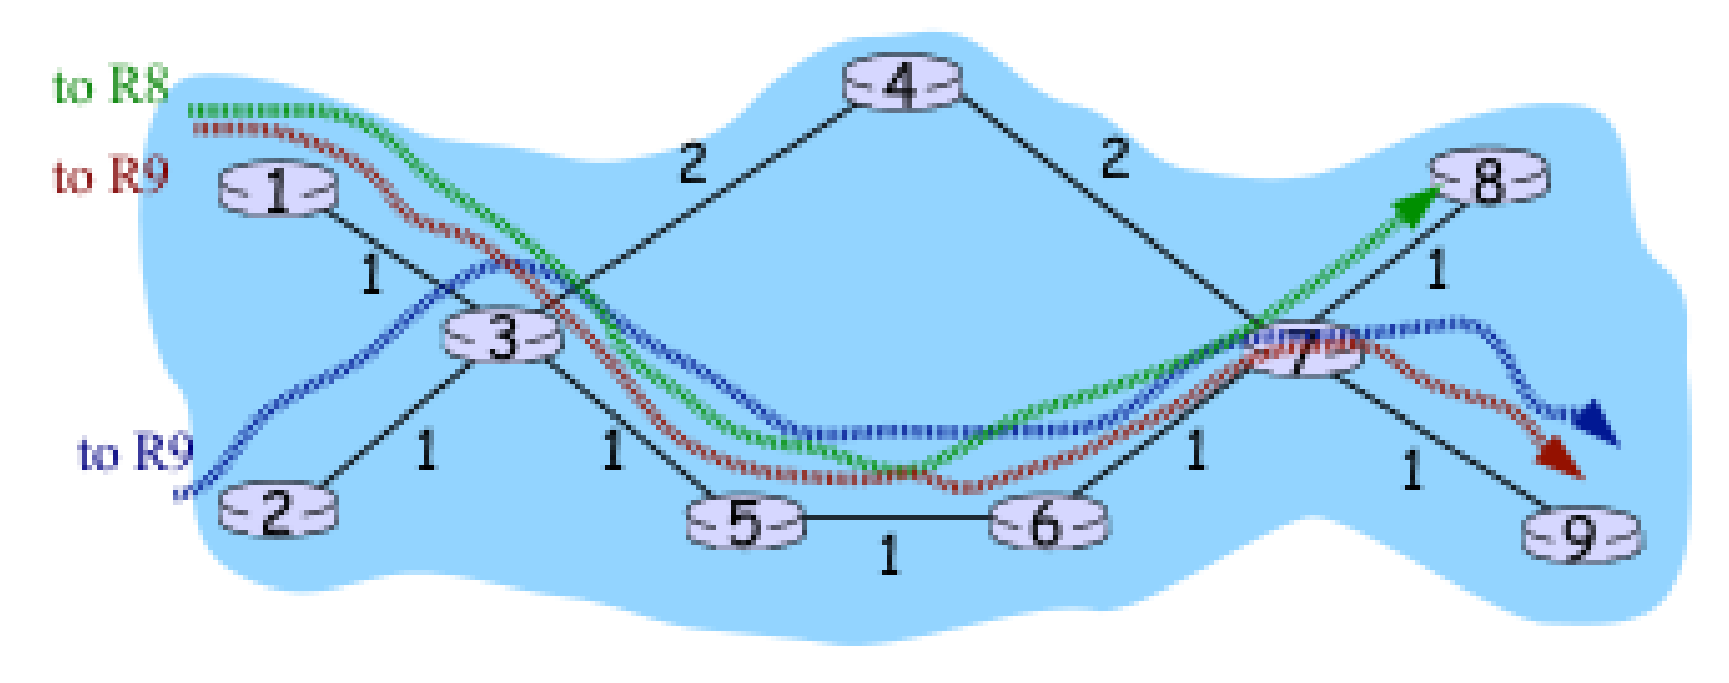
\includegraphics[width=\textwidth]{fishnetwork.eps}

Comment pourrais-t-on mieux utiliser le réseau ?

\paragraph{ECMP (Equal-cost Multiple Paths)}

Si plusieurs chemins de même coût sont disponibles:

\begin{itemize}
\item Simple balance de charge: On installe les chemins dans la FIB
  pour utiliser au mieux les resources
\item round-robin, facile à implémenter, répartit bien la charge
  \textbf{mais} deux paquets d'une même connexion TCP pourraient être
  envoyés sur deux chemins différents, causant ainsi du
  ré-ordonnancement et affectant gravement le traffic
\item pour chaque nouveau flux TCP, choisir un chemin et le retenir
  pour les paquets suivants du même flux (problèmes: il faut stocker
  tout cela en mémoire, il faut faire des lookups rapidement dans ces
  données)
\item fonction de hashage, même principe que la technique précédente
  mais pas d'état à retenir, plus rapîde et plus efficace.
\end{itemize}

Limitations pour les ECMP: marche mieux s'il y a beaucoup de petits
flux que s'il y a quelques énormes flux, marche mieux également s'il y
a beaucoup d'ECMP dans le réseau (cela dépend de la stratégie
d'assignation des poids des liens)

\paragraph{Stratégies d'assignation des poids des liens}

\begin{itemize}
\item Unitaire: chaque lien a un poids de 1, cela favorise les chemins
  avec peu de hops, et donne en général lieu à beaucoup d'ECMP.
\item Proportionnel à la latence du lien: favorise les chemins avec
  des délai court, mais limite le nombre d'ECMP en général
\item Proportionnel à l'inverse de la bande passante: par défaut sur
  les routeurs CISCO, favorise les chemins avec une large bande
  passante et les ECMP.
\item Sélection manuelle des poids sur chaque lien: se fait à l'aide
  d'outils pour balancer la charge de trafic.
\end{itemize}

\chapter{BGP}

\section{Routage inter-domaine}

\subsection{Objectifs fondamentaux}

\begin{itemize}
\item Permettre de transmettre des paquets IP par le meilleur chemin
  lorsqu'il est nécessaire de passer par plusieurs domaines de transit
  (souvent, ``meilleur chemin'' revient à ``chemin le moins cher'')
\item Prendre en compte les politiques de routage de chaque domaine
\item Autonomie (à l'intérieur d'un domaine, les opérations sont
  effectuées indépendamment des autres, chaque domaine peut faire
  tourner son propre IGP)
\item Cacher la topologie détaillée des domaines de transit (routage
  hiérarchique, nécessaire car le graphe inter-domaines possède des
  millions de noeuds)
\end{itemize}

\subsection{Définitions}

\begin{itemize}
\item Un système autonome (AS) est un réseau sous l'administration
  d'une entité unique (BELNET, Abilène, ...)
\item Un préfixe est un ensemble d'adresses IP spécifié dans la
  notation CIDR (193.190.192/22 (UMons), ...)
\item Lien privé: câble reliant deux routeurs appartenant à deux AS
  différents
\item Connection via un point d'interconnexion: En général via un
  switch Gigabit (ou plus)
\end{itemize}

\subsection{Politiques de routage}

Il y a deux politiques principales:

Un lien client-vendeur (un client C achète de la connectivité internet
à un provider P)

Un lien à coût partagé (les domaines X et Y se mettent d'accord pour
échanger des paquets en utilisant un lien direct ou un point
d'interconnexion)

Bien sûr, des politiques plus complexes sont possibles (et existent)

\paragraph{Matrice de politique de transit}

\begin{tabular}{c|c|c|c|c|}
  \multicolumn{2}{c|}{} & \multicolumn{3}{c|}{Vers} \\
  \cline{3-5}
  \multicolumn{2}{c|}{} & Provider & Pair & Client \\
  \hline
  \multirow{3}{*}{De} & Provider & \color{red}{Non} & \color{red}{Non} &
     \color{green}{Oui} \\
  \cline{2-5}
  & Pair & \color{red}{Non} & \color{red}{Non} & \color{green}{Oui} \\
  \cline{2-5}
  & Client & \color{green}{Oui} & \color{green}{Oui} & \color{green}{Oui} \\
  \hline
\end{tabular}

\paragraph{RPSL}

Pour faire appliquer ces règles (ou d'autres), un mécanisme de filtres
est mis en place. Les administrateurs de réseaux peuvent donc
appliquer un ou plusieurs filtres à chaque ``porte'' de leur réseaux:
des filtres d'imports, qui permettent de limiter le trafic entrant, et
des filtres d'export, qui permettent de limiter le trafic sortant.

Ces filtres sont en général exprimés dans un langage spécifique au
vendeur du routeur, le standard est RPSL (Routing Policy Specification
Language)

Exemples simples de syntaxe RPSL:

\begin{verbatim}
import: from AS# accept list_of_AS

import: from BELNET accept UMONS
import: from LEVEL3 accept ANY

export: to AS# announce list_of_AS

export: to UMONS announce ANY
export: to LEVEL3 announce UMONS UCLOUVAIN ...
\end{verbatim}

\section{BGP}

\subsection{Principes}

Il s'agit du standard pour le routage inter-domaines

Permet à chaque AS ...

\begin{itemize}
\item ... de savoir si tel ou tel préfixe peut être atteint depuis les
  AS voisins
\item ... de propager cette information dans chaque routeur interne à
  l'AS
\item ... de déterminer les ``bonnes'' routes vers les sous-réseaux en
  se basant sur l'information d'atteignabilité et la politique de
  l'AS.
\end{itemize}

BGP permet également aux sous-réseaux de signaler leur existence.

Pour remplir ces objectifs, BGP utilise un protocole de vecteurs de
distance et des mises à jour incrémentales. (Avertisement de mise à
jour seulement quand l'information change)

\subsection{Sessions}

\paragraph{Principe}

Les paires de routeurs BGP s'échangent des routes sur leur connexion
TCP semi-permanente: la session BGP

Les routeurs disposant d'une session BGP sont appelés pairs BGP ou
voisins BGP.

Le port par défaut pour les sessions BGP est 179.

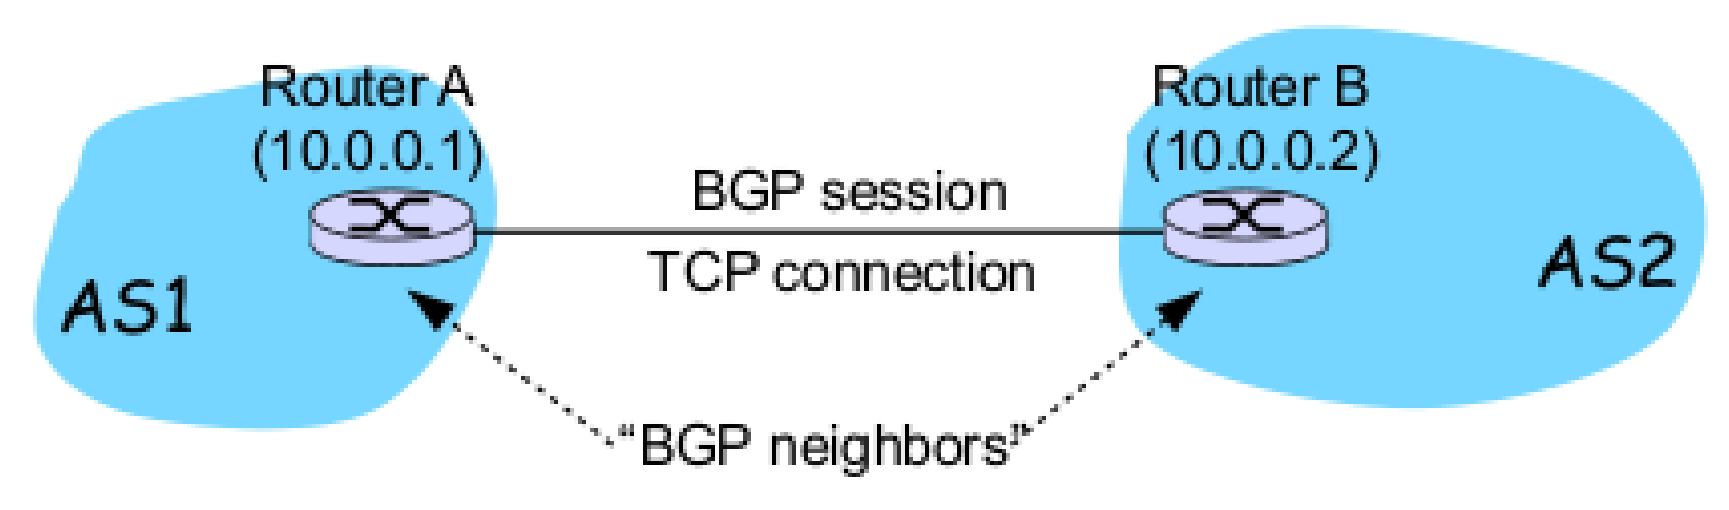
\includegraphics[width=\textwidth]{bgpsession.eps}

\paragraph{Configuration d'une session BGP}

Préliminaire: les deux routeurs doivent être capables de s'atteindre

CISCO:

\begin{verbatim}
# router bgp [ASN]
# neighbor [IP_VOISIN] remote-as [ASN_VOISIN]
\end{verbatim}

Juniper:

\begin{verbatim}
routing-options {
  autonomous-system [ASN];
}

protocols {
  bgp {
    group [NOM_GROUPE_VOISINS] {
      peer-as [ASN_VOISIN];
      type external;
      neighbor [IP_VOISIN];
    }
  }
}
\end{verbatim}

\subsection{Messages}

4 grands types de messages dans le protocole BGP:

\begin{itemize}
\item OPEN (ouverture de session, éventuellement authentification)
\item UPDATE (avertissement des chemins neufs / obsolètes)
\item KEEPALIVE (maintient une connexion, ack du OPEN)
\item NOTIFICATION (erreurs, fermeture de connexion)
\end{itemize}

Le header d'un message BGP est composé des champs suivants:

\begin{itemize}
\item Marker (16 bytes) inutilisé, ne doit contenir que des 1
\item Longueur (2 bytes) longueur du paquet, header compris
\item Type (1 byte) 1=OPEN, 2=UPDATE, 3=NOTIFICATION, 4=KEEPALIVE,
  5=ROUTE REFRESH
\item Corps du message
\end{itemize}

\paragraph{Message OPEN}

Le corps est composé des champs suivants:

\begin{itemize}
\item Version (1 byte) vaut 4 (00000100)
\item ASN de l'émetteur (2 bytes)
\item Temps d'attente (2 bytes)
\item Identifiant BGP (4 bytes) Adresse IP d'une des interfaces du
  routeur émetteur
\item Longueur des paramètres optionnels (1 byte)
\item Paramètres optionnels (triplets [type, longueur, valeur])
\end{itemize}

\paragraph{Message UPDATE}

Le corps est composé des champs suivants:

\begin{itemize}
\item Nombre de routes obsolètes (2 bytes)
\item Routes obsolète (variable)
\item Longueur des attributs de chemins (2 bytes)
\item Attributs de chemins (variable)
\item Network Layer Reachability Information [NLRI] (variable)
\end{itemize}

\subsection{Routes}

\paragraph{Définition}

Une route est la combinaison d'un préfixe de destination et
d'attributs de chemin, elle est transportée par un message UPDATE, le
préfixe de destination est spécifié dans la partie NLRI du message et
un routeur BGP annonce une seule route par préfixe de destination.

\paragraph{Avertissements de routes}

Ils proviennent de diverses sources:

\begin{itemize}
\item Routes statiques, configurées manuellement dans le routeur
\item Redistribution de route (apprises par un protocole de routage
  intra-domaine, iBGP par exemple), mais c'est une mauvaise habitude
  vu que les instabilités intra-domaine seraient répercutées à
  l'extérieur et risqueraient de rendre le BGP global instable
\item Apprentissage de routes depuis un autre routeur BGP (chaque
  noeud BGP avertit ses voisins de ses meilleures routes)
\end{itemize}

\paragraph{Abandon de routes}

Principe: quand une destination n'est plus atteignable, un routeur BGP
doit en avertir ses voisins.

Les messages UPDATE sont utilisés pour informer qu'une route n'est
plus disponible, on appelle ces messages WITHDRAW alors que,
strictement, aucun message WITHDRAW n'existe dans la spécification
BGP. Un WITHDRAW ne doit être envoyé que pour des routes précédemment
annoncées.

Un WITHDRAW implicite est un message UPDATE modifiant juste un
attribut de la route (c'est-à-dire que la destination peut toujour
être atteinte, mais avec d'autres paramètres car il faut passer par
d'autres routeurs BGP par exemple).

\subsection{Attributs des chemins}

Une route peut contenir plusieurs attributs; les deux les plus
importants sont NEXT-HOP (IP du prochain routeur BGP sur la route) et
AS-PATH (liste des ASN des routeurs suivants sur la route)

L'AS-PATH, en plus de servir de métrique, permet d'éviter les boucles
de routage: un routeur BGP voyant son propre ASN dans l'AS-PATH ne
considérera pas cette route.

Attributs de chemins standardisés

\begin{tabular}{l|c|c|c|c|c|}
  Nom & Code & Implémentation & attribut & Transitif \\
  & & obligatoire & obligatoire & \\
  \hline
  ORIGIN & 1 & Y & Y &  \\
  \hline
  AS-PATH & 2 & Y & Y & \\
  \hline
  NEXT-HOP & 3 & Y & Y & \\
  \hline
  MED (Multi Exit Discriminator) & 4 & & & \\
  \hline
  LOCAL\_PREF & 5 & Y & & \\
  \hline
  ATOMIC\_AGGREGATE & 6 & Y & & \\
  \hline
  AGGREGATOR & 7 & & & Y \\
  \hline
  COMMUNITIES & 8 & & & Y \\
  \hline
  ORIGINATOR\_ID & 9 & & & \\
  \hline
  CLUSTER\_LIST & 10 & & & \\
  \hline
  EXTENDED\_COMMUNITIES & 16 & & & \\
  \hline
\end{tabular}

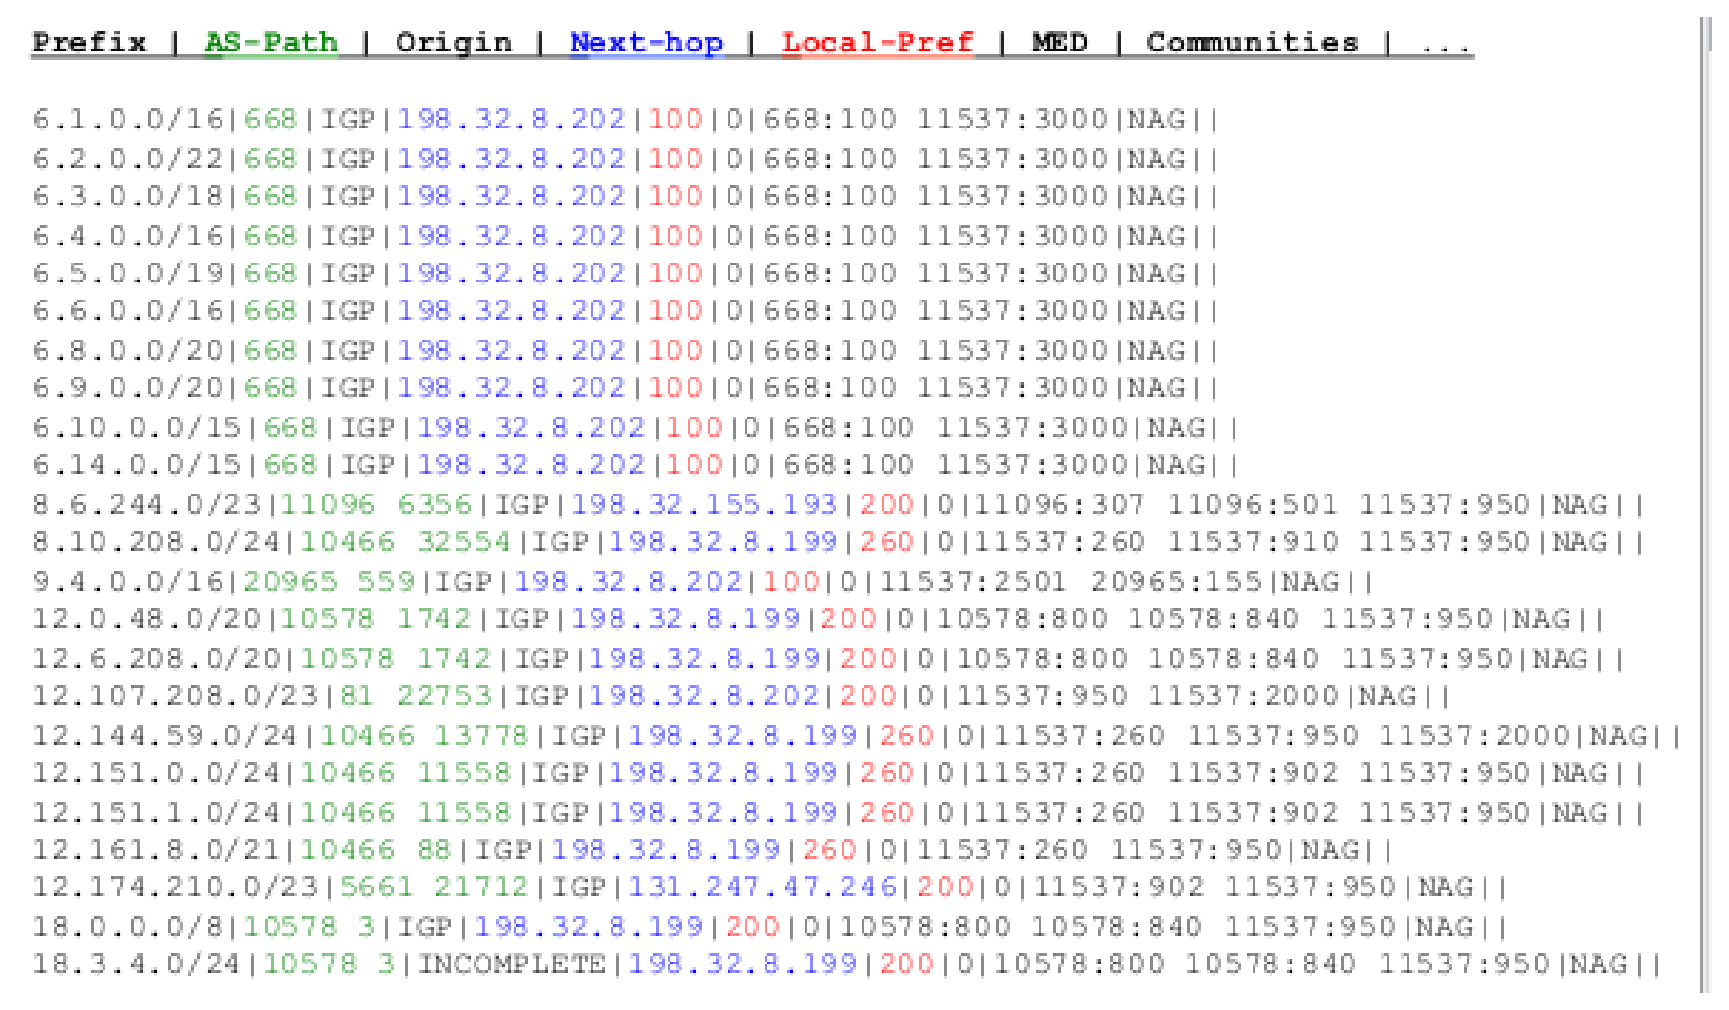
\includegraphics[width=\textwidth]{bgproutesconfig.eps}

\subsection{Machine à états finie}

Le but de la machine à étatss BGP est de s'assurer de la gestion
correcte des messages BGP comme de la robustesse des sessions
BGP. Toute implémentation pour un routeur BGP doit suivre le même
comportement que la machine à états.

La machine est composée de 6 états:

\begin{itemize}
\item Idle (état initial)
\item Connect (tentative d'initiation de connexion TCP)
\item Active (écoute de connexions TCP entrantes)
\item OpenSent (OPEN envoyé, attente d'un OPEN entrant)
\item OpenConfirm (OPEN reçu, KEEPALIVE envoyé, attente d'un KEEPALIVE
  entrant)
\item Established (En marche, échange de KEEPALIVE et de UPDATE)
\end{itemize}

Et de 3 timers:

\begin{itemize}
\item ConnRetry (Espace les tentatives de connexion TCP)
\item HoldTimer (Assure l'activité de la session BGP)
\item KeepAlive (Envoie des KEEPALIVE régulièrement)
\end{itemize}

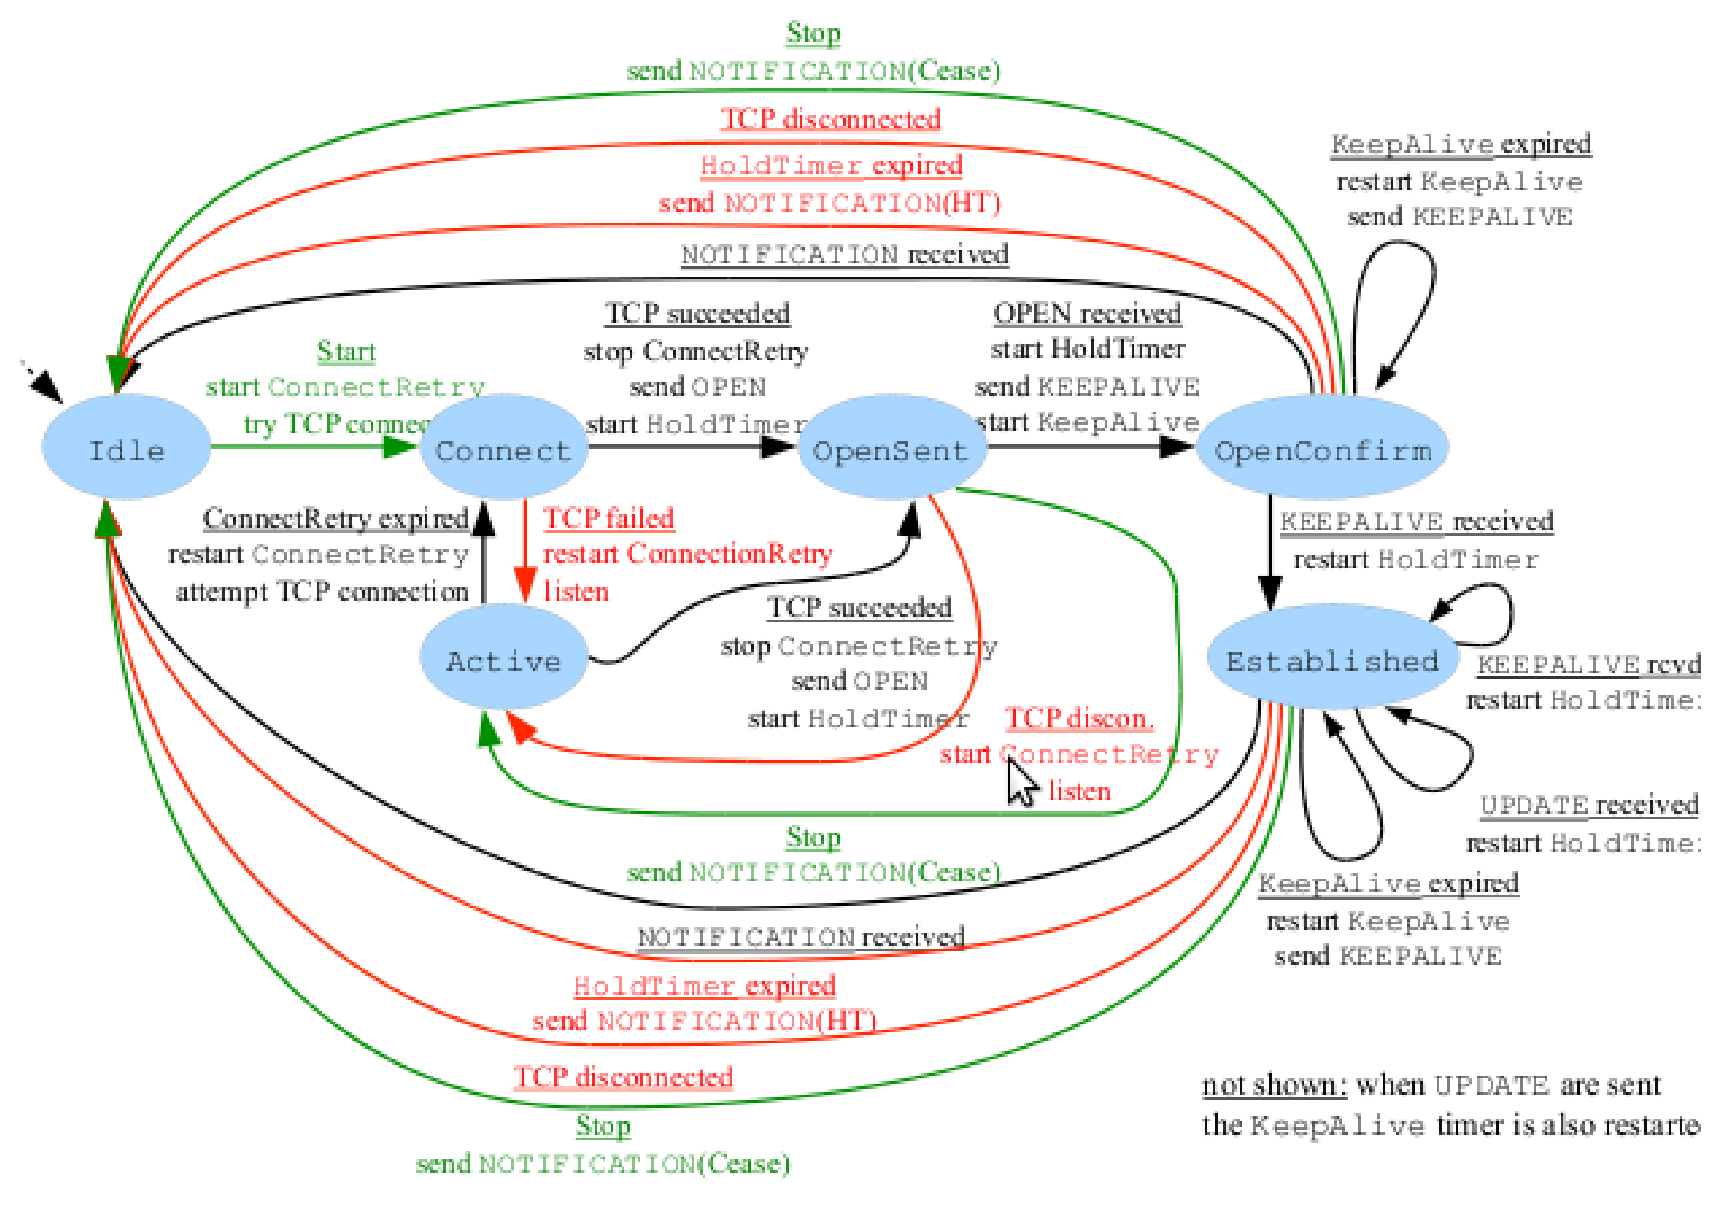
\includegraphics[width=\textwidth]{bgpmachine.eps}

\subsection{Processus de décision}

Un routeur recevra souvent plusieurs routes pour joindre un même
préfixe. Il doit alors choisir une unique meilleure route à
communiquer à ses voisins.

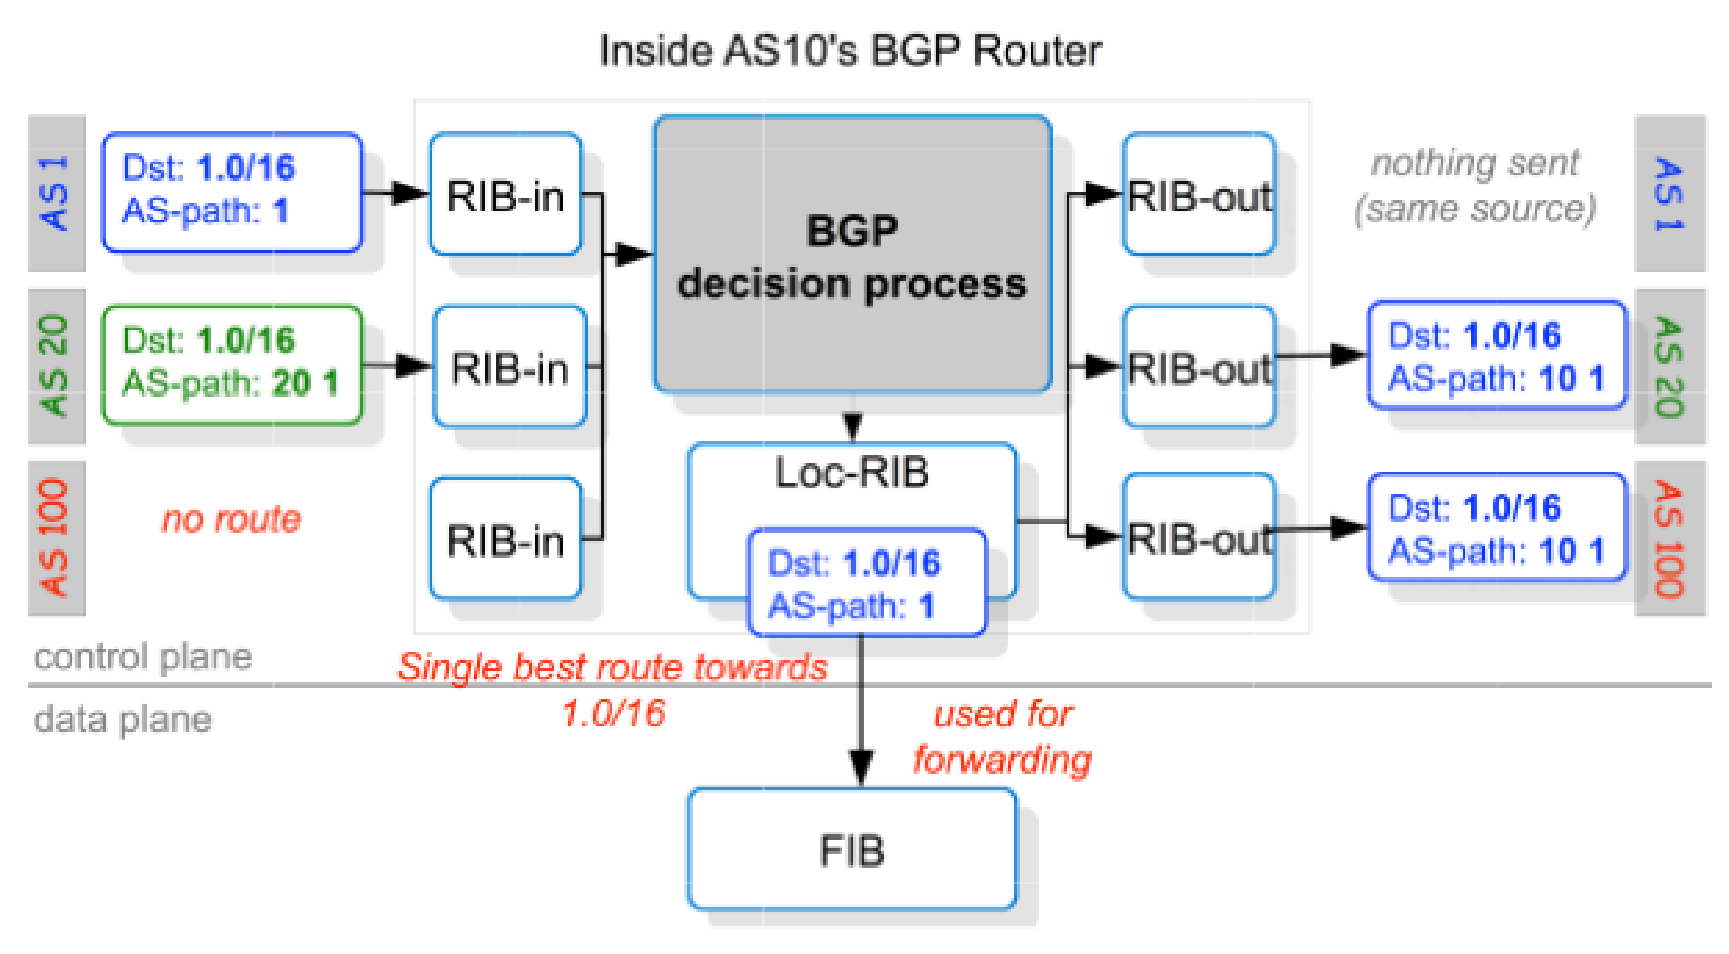
\includegraphics[width=\textwidth]{decisionprocess.eps}

Le processus de décision est composé d'une série de règles qui va
réduire l'ensemble des routes admissibles pour un préfixe donné
jusqu'à ce qu'il n'en reste qu'une, ce sera la meilleure route, qui
sera ensuite communiquée aux voisins du routeur (en accord avec la
politique de l'AS bien entendu).

Le processus simplifié ressemble à ceci:

\begin{itemize}
\item Ignorer si le NEXT-HOP n'est pas joignable
\item Préférer les routes ayant un LOCAL-PREF supérieur
\item Préférer les routes ayant un AS-PATH plus court
\item Tie-break
\end{itemize}

Voici le processus de décision complet:

\begin{enumerate}
\item Ignorer si le NEXT-HOP n'est pas joignable
\item Préférer les réseaux originaires du réseau local
\item Préférer les routes ayant un LOCAL-PREF supérieur
\item Préférer les routes ayant un AS-PATH plus court
\item Préferer les ORIGIN les plus bas
\item Préférer les MED les plus bas
\item Préférer eBGP par rapport à iBGP
\item Préférer le NEXT-HOP le plus proche
\item Préférer le ROUTER-ID / ORIGINATOR-ID le plus bas
\item Préférer le CLUSTER-LIST le plus court
\item Préférer l'adresse du voisin la plus petite
\end{enumerate}

On s'en doute, les trois derniers points sont des tie-breaks.

\subsection{Filtres de routage}

\paragraph{Objectifs}

\begin{itemize}
\item Influencer le classement des routes
\item Empêcher certaines routes d'être redistribuées à certains voisins
\item Rejeter une route d'un voisin spécifique
\end{itemize}

\paragraph{Principes}

\begin{itemize}
\item Ajouter des filtres d'import/export au modèle de routage BGP
  pour chaque voisin
\item Filtres d'import (in-filters): sélectionner les routes
  acceptables et changer leurs attributs
\item Filtres d'export (out-filters): sélectionner les routes
  redistribuables et changer leurs attributs
\item Les filtres sont spécifiés dans un langage spécifique au vendeur
  du matériel
\end{itemize}

Un filtre est un ensemble de prédicats qui mènent à un ensemble
d'actions.

\paragraph{Exemples de prédicats}

\begin{itemize}
\item match destination prefix against IP prefix
\item match next-hop against IP address / prefix
\item test existence of an ASN in AS-PATH
\item match AS-PATH against regular expression
\item ...
\end{itemize}

\paragraph{Exemples d'actions}

\begin{itemize}
\item Accept / reject the route
\item Set / Increase / Decrease LOCAL-PREF
\item Prepend AS-PATH
\item Set MED
\item Add / Remove community
\item Remove private ASN from AS-PATH
\item ...
\end{itemize}

\paragraph{Exemple d'application}

Un AS possède souvent plusieurs liens vers son provider. Un lien
principal qui doit être utilisé autant que possible et un lien
secondaire qui doit être utilisé lorsque le lien secondaire ne
fonctionne pas.

On peut donc configurer un filtre donnant une priorité plus grande aux
routes fournies par le routeur de la route principale

\begin{verbatim}
import: from AS2 RB at RA set localpref=200;
import: from AS2 RC at RA set localpref=100;
\end{verbatim}

Cela aura pour effet de donner une priorité plus grandes aux routes
fournies par le routeur RB, alors qu'elles sont en fait équivalentes à
celles fournies par le routeur RC en termes d'étendue (pas forcément
en termes de rapidité / bande passante)

\paragraph{Autre exemple d'application}

L'attribut LOCAL-PREF est souvent utilisé pour représenter les
relations économiques entre les AS, elles sont définies de telle sorte
qu'on ait:

\[rank(customer routes) > rank(peer routes) > rank(provider routes)\]

Remarquons que cela permet l'utilisation de routes asymétriques pour
l'aller et le retour, comme l'illustre le schéma suivant:

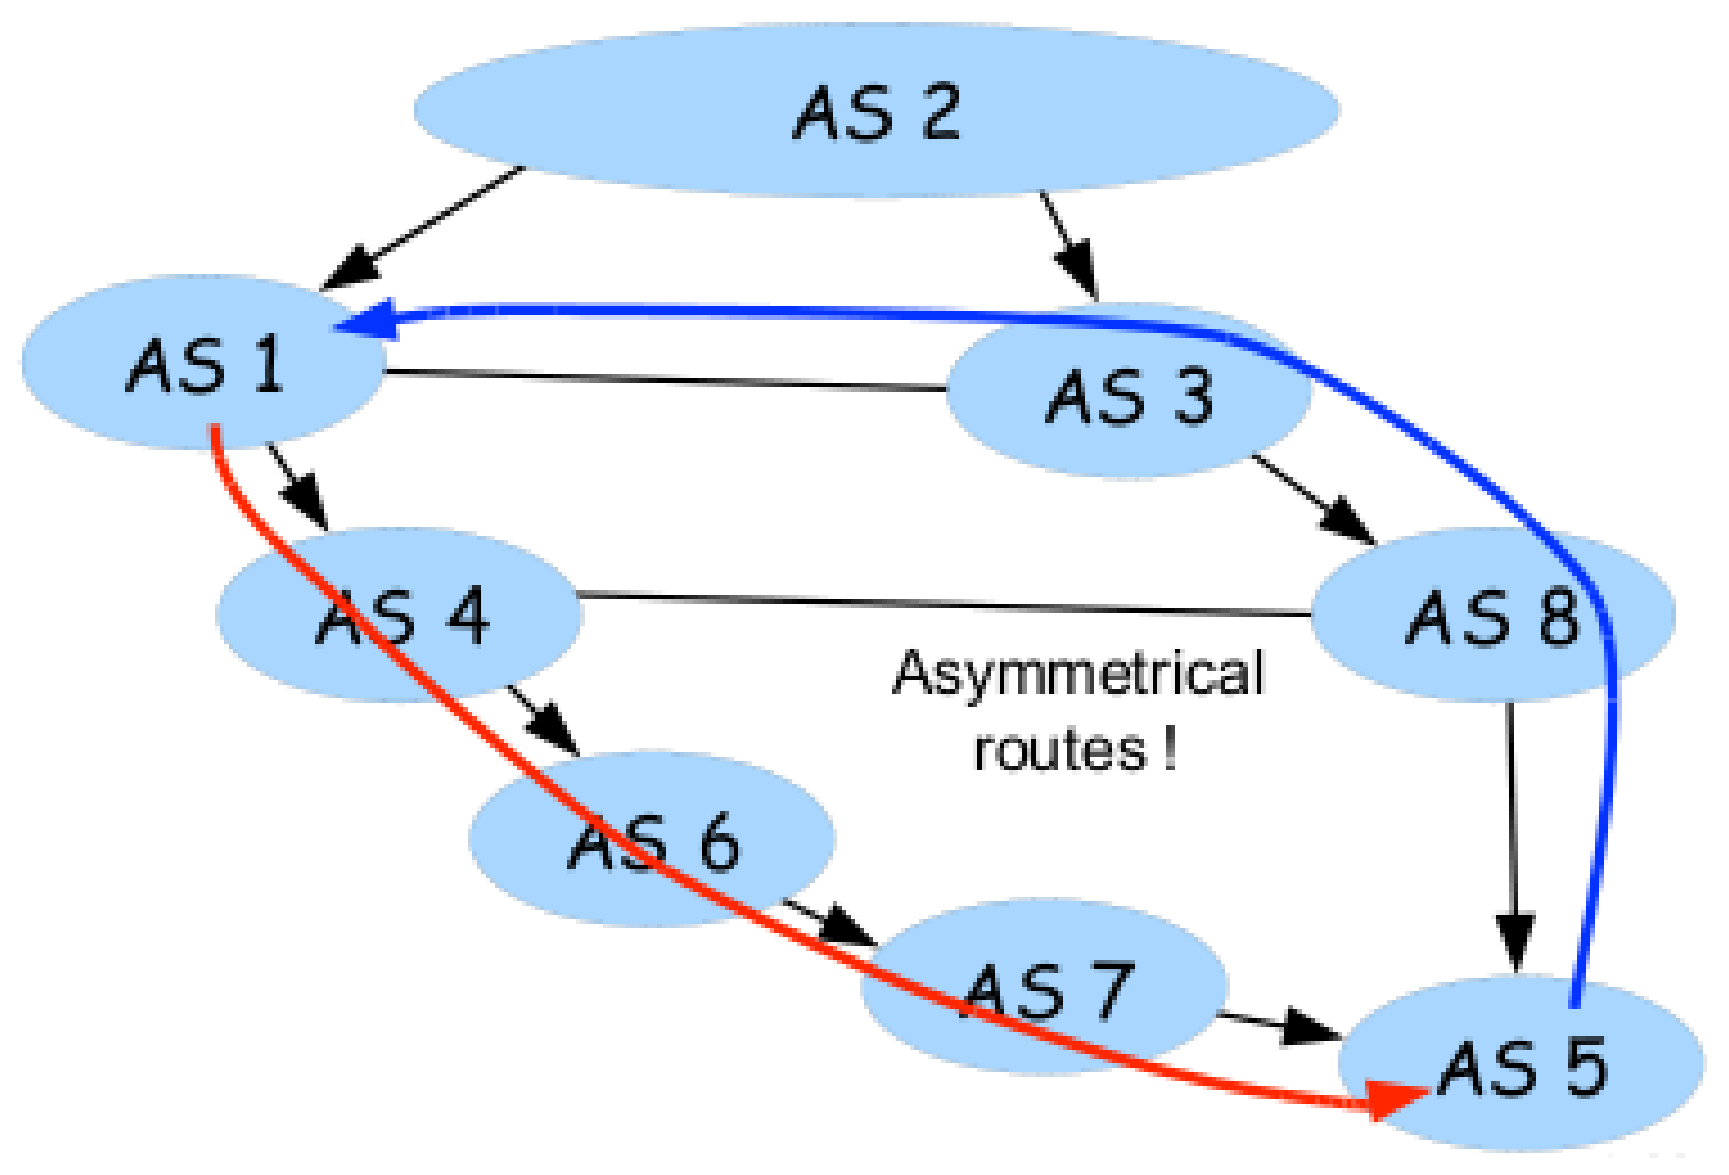
\includegraphics[width=\textwidth]{asymetricalroutes.eps}

Dans cet exemple, les paquets devant aller de AS8 à AS1 ne passent pas
par AS4 (c'est pourtant plus avantageux pour AS8 !) car AS4 n'a pas
annoncé qu'il avait une route vers AS1 à AS8.

\paragraph{Filtres automatiques du protocole}

En plus des filtres définis par la configuration, les routeurs BGP
appliquent les filtres suivans automatiquement:

\begin{itemize}
\item LOCAL-PREF est enlevé des routes avant qu'elles soient transmises
\item L'ASN du routeur est ajoutée au début de l'AS-PATH des routes
  avant qu'elles soient transmises
\item Une route contenant l'ASN d'un voisin ne sera pas transmise à ce
  voisin (sender-side loop detection)
\item l'attribut NEXT-HOP est mis à jour avant que la route ne soit
  transmise
\end{itemize}

\subsection{BGP interne (iBGP)}

iBGP permet aux routeurs d'un AS de s'échanger des routes, il s'agit
en fait d'une version modifiée de BGP dont les principales différences
sont:

\begin{itemize}
\item LOCAL-PREF n'est transporté que sur les sessions iBGP (pas eBGP)
\item les filtres d'import/export ne sont définis que pour les
  sessions eBGP
\item les routes apprises dans les sessions iBGP ne peuvent pas être
  redistribuées sur d'autres sessions iBGP
\item les attributs NEXT-HOP et AS-PATH ne sont mis à jour que lorsqu
  la route est envoyée à travers une session eBGP
\end{itemize}

Afin que tout se passe bien dans l'AS, il est préférable que tous les
routeurs internes fassent tourner BGP (on appelle cela un full mesh).

Sinon, on peut:

\begin{itemize}
\item utilier des tunnels (MTU réduit, routeurs ``chargés'' par
  l'encapsulation/décapsulation des paquets aux extrémités du tunnel,
  configuration statique nécessaire (manuelle))
\item redistribuer les routes BGP dans l'IGP (très mauvais pour la
  montée en charge, danger de réinjecter les routes dans BGP avec un
  AS-PATH de longueur unitaire (AS7007)
\end{itemize}

\paragraph{En résumé}

Le rôle d'IGP est de distribuer la topologie interne et les adresses
internes à l'intérieur de l'AS, tandis que le rôle d'iBGP est de
distribuer les routes vers les destinations extérieures apprises par
eBGP aux autres routeurs de l'AS.

Les sessions iBGP peuvent être établies grâce aux route IGP.

\paragraph{Préférer eBGP à iBGP dans le processus de décision}

Aussi appelé ``routage de la patate chaude'', un routeur devrait
tenter de se débarasser des paquets à destination d'autres domaines
(AS) aussi rapidement que possible.

\paragraph{Choisir le next-hop le plus proche}

Toujours dans l'optique du ``routage de la patate chaude'', lorsque
les règles précédentes du processus de décision amènent à des
égalités, on utilise le next-hop (IGP, s'entend) le plus proche.

\paragraph{Choisir le MED le plus faible}

Alors que les deux règles qu'on vient de voir favorisent l'émetteur
des paquets, le MED permet au futur récepteur d'influencer l'émetteur
sur la route à choisir. Cependant l'émetteur peut choisir de
simplement ignorer le MED. Celui qui annonce une route vers un certain
préfixe peut ainsi joindre à la route un MED indiquant quelle route il
préfère à une autre (plus le MED est faible, plus la route est
favorable pour l'annonceur de la route)

Le MED impose toutefois un problème supplémentaire: deux MED ne
peuvent être comparés que si les routes auxquelles ils appartiennent
proviennent du même AS.

La règle ``Choisir le MED la plus faible'' dans le processus de
décision va donc consister à garder, pour chaque AS ayant encore des
routes ``en lice'', celle ayant le MED le plus faible.

\section{Ingénierie de trafic basée sur BGP}

\subsection{Multi-homing}

Au début de sa vie, un AS, connecté à un seul provider, utilise un ASN
privé (de 64512 à 65535) et est complètement caché derrière son ISP.

Ensuite, l'AS veut devenir multi-homed et obtient un ASN public. l'ISP
doit alors prévenir ses autres clients qu'un nouvel AS existe et faire
ainsi grossir la taille des tables de routage globales.

\paragraph{Aggrégation}

BGP peut agréger les routes reçues, l'attribut AS-PATH est une
AS-séquence formée d'AS-ensembles, la plupart des AS-ensembles sont
constitués d'un seul élément, Un AS-ensemble n'est pas ordonné et
compte pour une longueur de 1.

L'information sur le chemin réel est perdue lorsque les AS-ensembles
sont utilisés; mais l'aggrégation permet le diminution de la taille
des tables de routage. Une liste des ``mauvais élèves'' n'utilisant
pas l'aggrégation est maintenue. On estime que, si l'aggrégation était
parfaitement utilisée, on pourrait réduire de 50\% la taille des
tables de routage.

\paragraph{Revenons à notre AS, il devient multi-homed}

Comme son ISP initial utilisait l'aggrégation, et que le nouvel ISP ne
l'utilise pas (il ne peut pas, le préfixe du client n'entrant pas dans
son propre préfixe), l'AS-PATH proposé par le nouvel ISP sera toujours
utilisé (le préfixe est plus précis).

De son côté, l'ISP initial devrait arrêter d'agréger le préfixe du
client, sinon le client ne recevra pas les paquets des autres clients
agrégés (Le provider va annoncer une route contenant l'AS du client,
le client va donc la rejeter, et n'aura pas connaissance des routes
vers les autres clients du provider. Idem si les routes passent par
d'autres routeurs: l'AS du client restera dans l'AS-PATH et la route
sera donc systématiquement jetée (ou même pas reçue par le client avec
le sender-side loop detection)

\paragraph{Comment limiter l'expansion des tables de routage ?}

Sur le long terme, IPv6 apportera une solution, en définissant une
meilleure notion de multi-homing.

\subsection{Gestion du trafic via BGP}

On aimerait par exemple que le trafic vers un certain préfixe passe
par un fournisseur, tandis que le trafic vers un autre préfixe passe
par un autre fournisseur, ou alors privilégier un lien par rapport à
un autre, mais garder l'autre comme back-up. Plusieurs techniques sont
envisageables:

\begin{itemize}
\item Annonces sélectives: N'annoncer certain préfixes que sur
  certains liens (Expansion des tables de routage, que se passe-t-il
  si un lien lache ?)
\item Préfixes plus spécifiques: Annoncer un préfixe global sur chaque
  lien, et un préfixe plus spécifique sur chaque lien (Expansion des
  tables de routage, mais plus robuste)
\item AS-PATH prepending (rendre l'AS-PATH artificiellement plus long
  en ajoutant plusieurs fois son ASN à l'AS-PATH selon le lien sur
  lequel on se trouve à l'aide d'un filtre)
\end{itemize}

\section{Résistance à la montée en charge}

\paragraph{Objectifs}

\begin{itemize}
\item Réduire le nombre de sessions iBGP (full mesh !), deux
  techniques pour cela: les confédérations et la réflection de routes
\item Permettre une gestion des politiques de routage plus
  ``scalable'', la technique proposée est l'utilisation des
  communautés
\end{itemize}

\subsection{Confédérations}

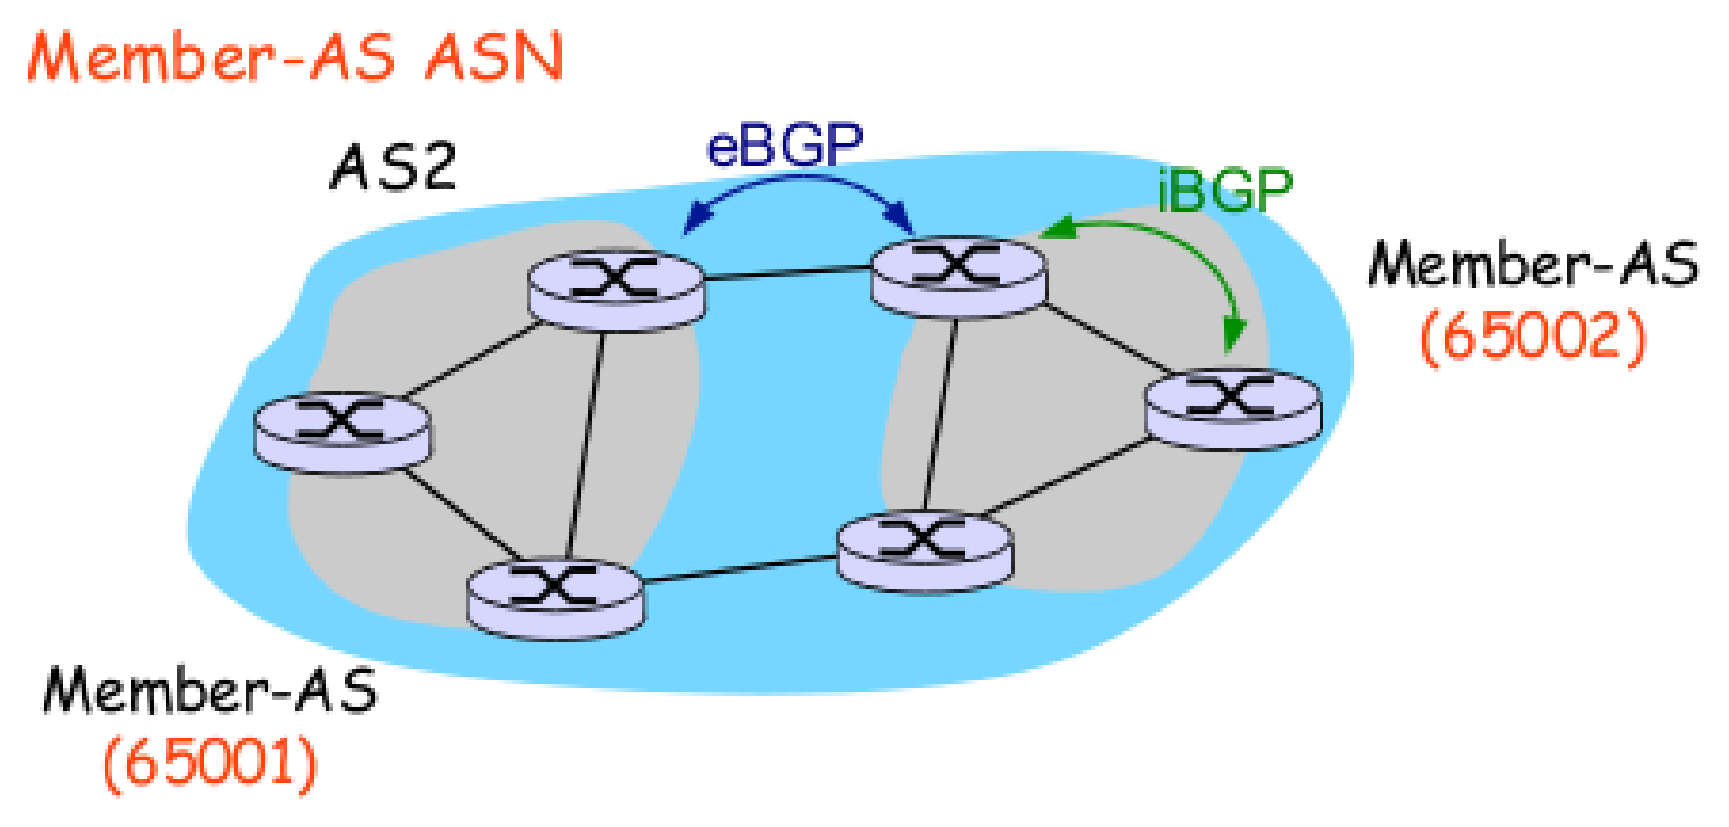
\includegraphics[width=\textwidth]{confederations.eps}

\begin{itemize}
\item iBGP est utilisé à l'intérieur de chaque AS-membre, eBGP est
  utilisé entre les AS-membres, chaque routeur a deux ASN: celui de la
  confédération et celui de l'AS-membre.
\item Suivant la session eBGP, un routeur appartient à l'AS-membre ou
  à la confédération.
\item Lors de la propagation d'un UPDATE via eBGP vers un routeur de
  la même confédération, un routeur insert son ASN-membre dans
  l'AS-PATH
\item Il est autorisé d'annoncer un NEXT-HOP inchangé ainsi que
  l'attribut LOCAL-PREF.
\item Lorsque qu'un UPDATE est propagé en dehors de la confédération
  via eBGP, le routeur doit d'abord enlever les ASN-membre et ajouter
  l'ASN de la confédération.
\end{itemize}

\subsection{Réflection de routes}

Des routeurs spéciaux appelés \textbf{réflecteurs de routes} peuvent
propager sur une session iBGP des routes reçues d'une autre session
iBGP.

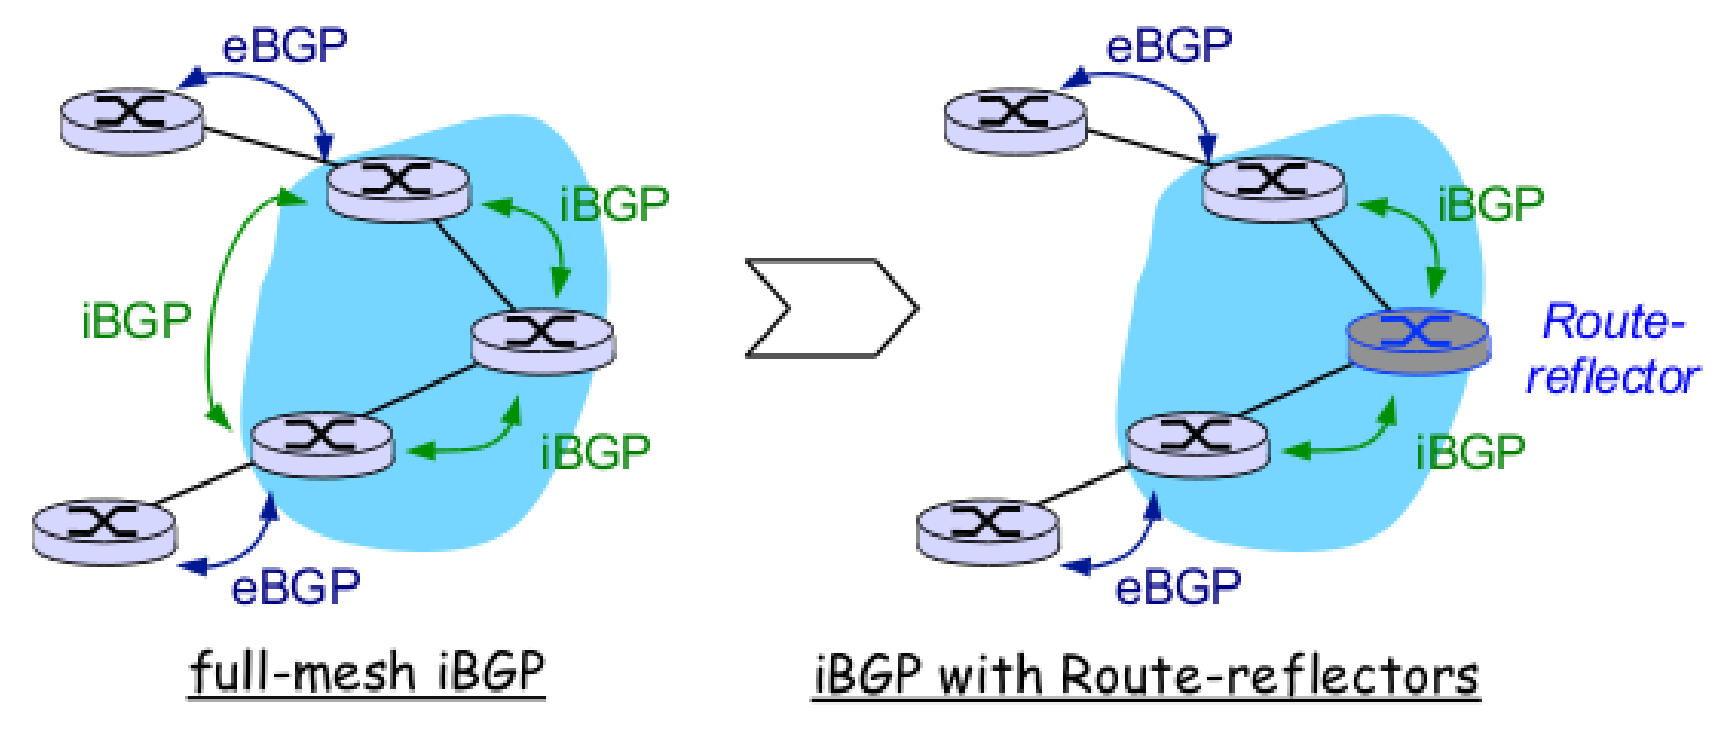
\includegraphics[width=\textwidth]{routereflection.eps}

Il y a deux types de noeuds iBGP quand il y a des RR: les noeuds
clients qui ne participent pas au full-mesh et les noeuds non-clients,
en full-mesh.

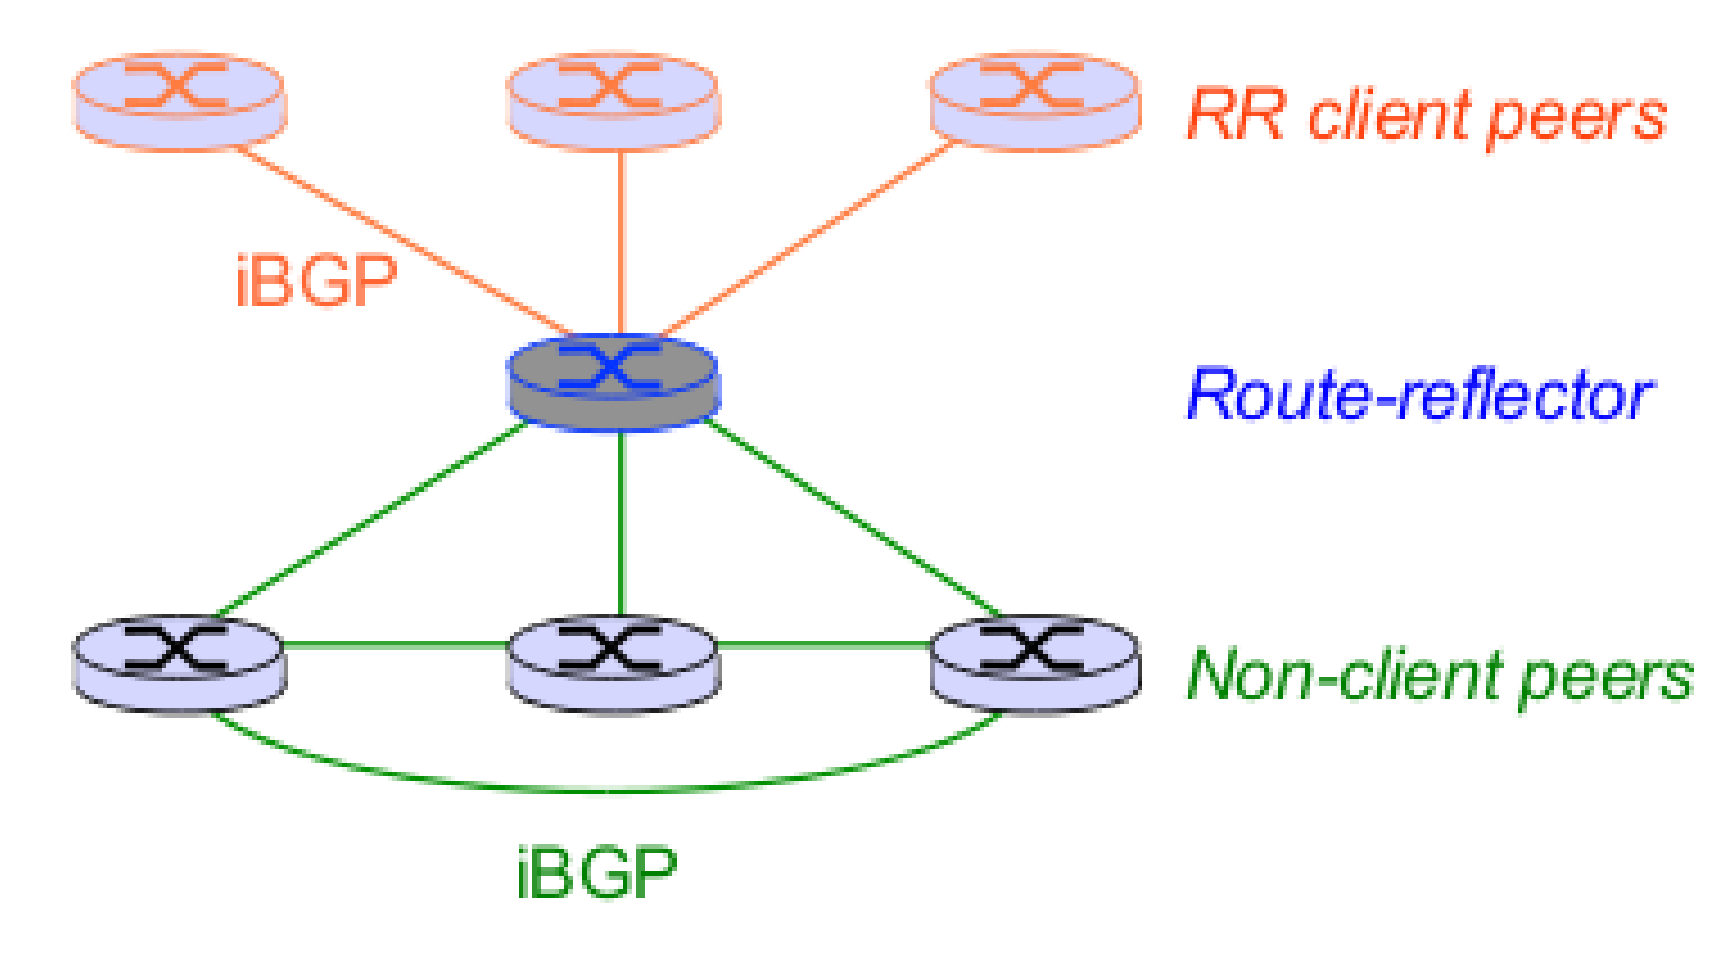
\includegraphics[width=\textwidth]{rrclients.eps}

Quand un RR reçoit une route d'un client ou de eBGP, il la redistribue
à tout le monde.

Quand un RR reçoit une route d'un non-client, il ne la redistribue
qu'aux clients.

\paragraph{Tolérance aux pannes}

Lorsque le RR tombe en panne, tous les clients sont déconnectés
(single point of failure). Pour éviter cela, chaque client est
connecté à au moins 2 RR.

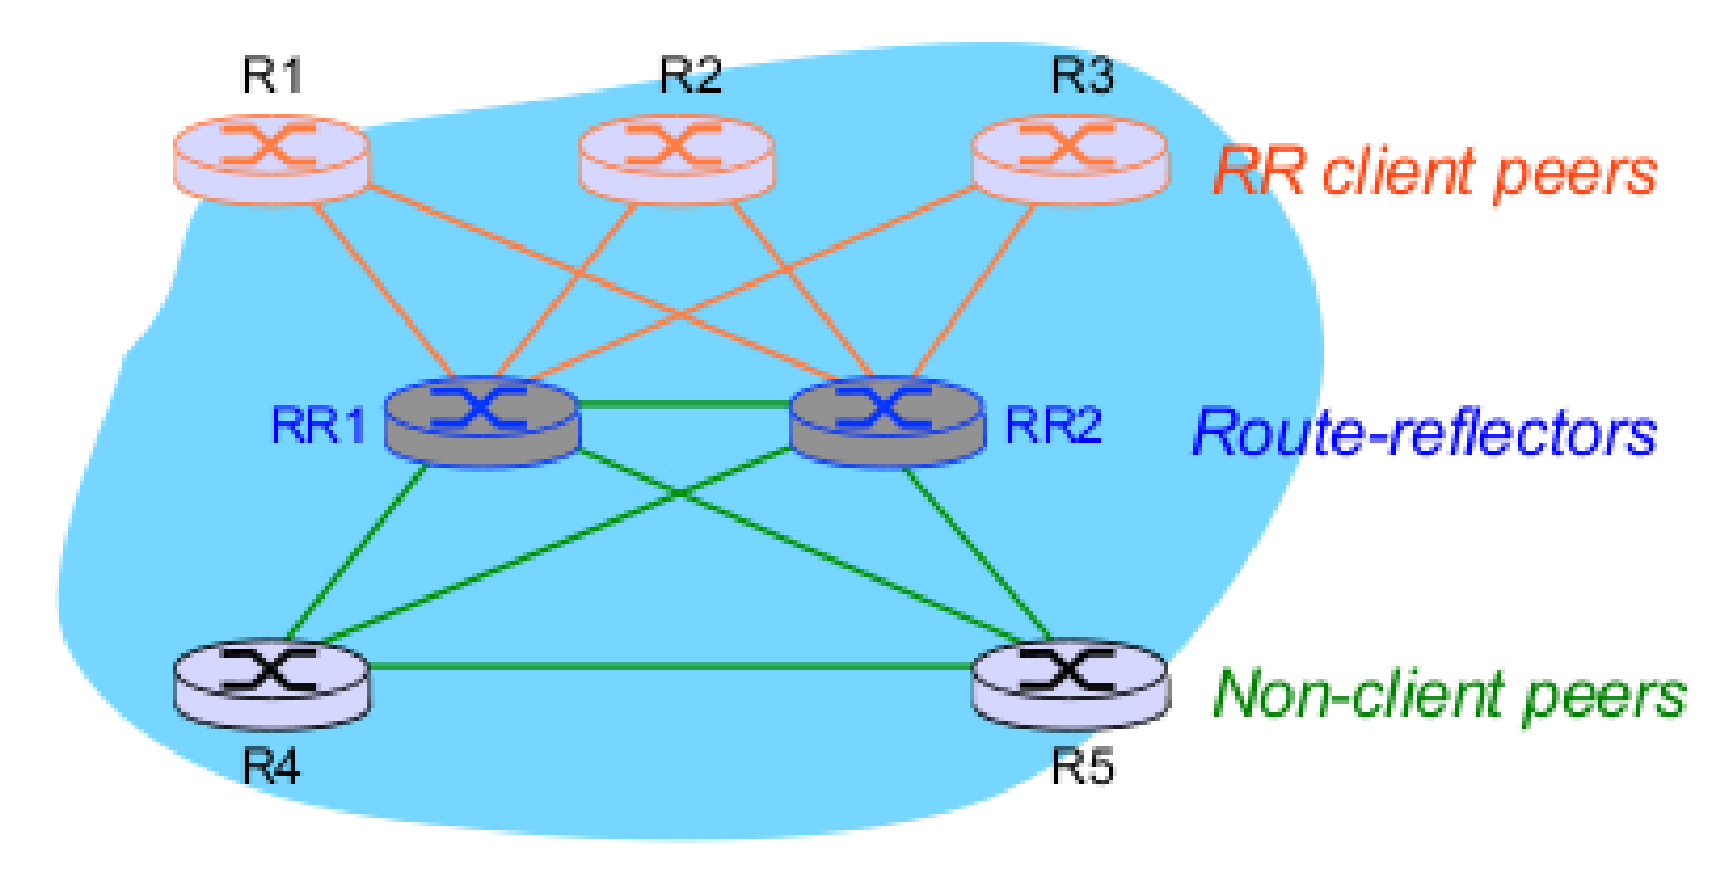
\includegraphics[width=\textwidth]{rrdual.eps}

\paragraph{Problème: les boucles de routage sont possibles}

Nous devons être sûr qu'un update ne peut être retourné à celui qui
l'a anoncé. Or, avec 2 RR, un client envoie l'UPDATE au premier RR,
qui le transmet au second, qui le renvoie au client (boucle).

La solution à ce problème est l'attribut BGP ORIGINATOR-ID. Quand un
RR réfléchit une route, il place l'identifiant du client qui a
envoyé la route dans l'ORIGINATOR-ID.

Les routeurs se voyant dans l'ORIGINATOR-ID refusent systématiquement
la route.

\paragraph{Hiérarchies de RR}

Un RR peut être lui-même client d'un autre RR, les mêmes règles de
redistribution des routes s'appliquent.

S'assurer que les boucles de routage sont impossibles devient moins
simple, ORIGINATOR-ID ne résoud plus ce problème.

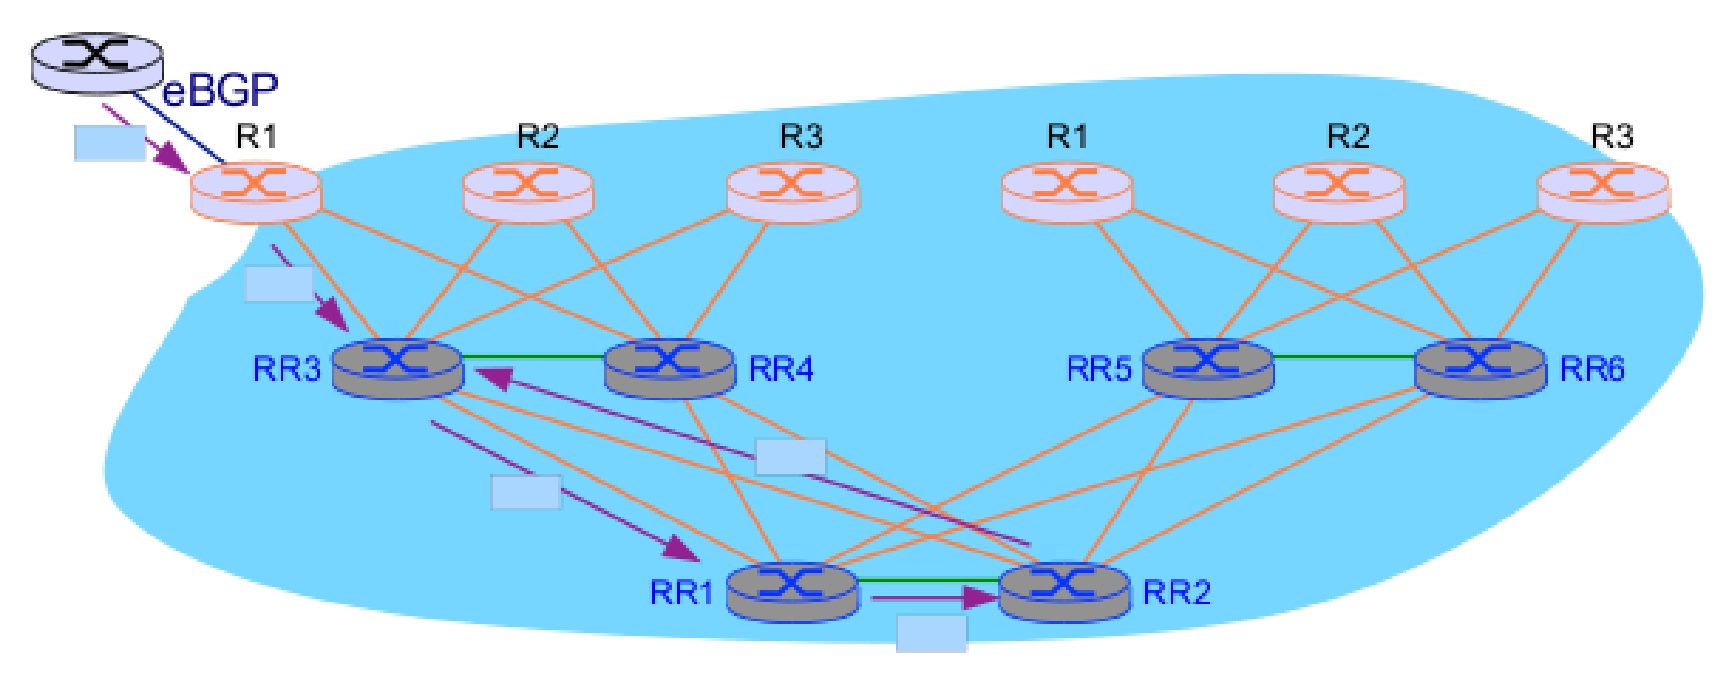
\includegraphics[width=\textwidth]{rrhierarchyloop.eps}

Comme réponse à ce problème, on introduit un nouvel attribut:
CLUSTER-ID-LIST; quand un RR réfléchit une route, il ajoute son propre
identifiant de cluster à la liste de la route.

Ensuite, pour éviter les boucles de routage, il suffit d'empêcher les
routes d'atteindre un cluster par lequel elle est déjà passée.

\paragraph{Processus de décision, règles 9 et 10}

On comprend à présent les tie-breaks 9 et 10 du processus de décision;
l'ORIGINATOR-ID et la CLUSTER-LIST proviennent en fait des clusters
lorsqu'on utilise les réflecteurs de routes.

\paragraph{Comparaison entre les RR et les confédérations}

Avec les RR, les clients ne doivent pas être au courant de la
hiérarchie, il suffit de configurer les RR, mais en contrepartie, la
charge de travail est très forte sur les RR, qu'on installe en général
sur les routeurs les plus puissants.

Avec les confédérations, il est simple de migrer d'une topologie
multi-AS vers une simple confédération (par exemple, lorsqu'une
société rachète une autre, elle peut vouloir intégrer le réseau de la
société achetée au sien avec le moins de coûts possible). Le point
noir des confédérations est que chaque routeur doit être configuré
pour connaître l'id de sa confédération et de son AS-membre.

\subsection{Filtres à grande échelle: les communautés}

Une communauté est une valeur entière spéciale qu'on peut attacher à
une route, elle est encodée sur 32 bits et deux routes avec la même
communauté attachée sont générallement traitées de la même manière.

Certaines valeurs de communauté sont standardisées, par exemple
$0xFFFFFF01$ (NO\_EXPORT) et $0xFFFFFF02$ (NO\_ADVERTISE).

Chaque AS dispose de 65536 valeurs de communautés pour lesquelles il
peut définir la sémantique qu'il souhaite (ASN:0000 $\rightarrow$
ASN:FFFF)

La valeur d'attribut BGP COMMUNITY contient une ensemble de valeurs de
communautés.

\paragraph{Exemple d'utilisation des communautés}

Souvent, les AS utilisent les communautés comme ceci: chaque routeur
en relation avec un client applique un filtre à toute les routes
reçues dont l'action est d'ajouter une communauté dont la valeur
signifie ``client'', de même pour les routeurs en relation avec des
pairs (valeur ``pair'') et les fournisseurs (valeur ``fournisseur'')

Ensuite, la politique peut être appliquée en fonction des communautés
plutôt qu'en fonction des routeurs, ce qui simplifie générallement le
travail des administrateurs réseaux.

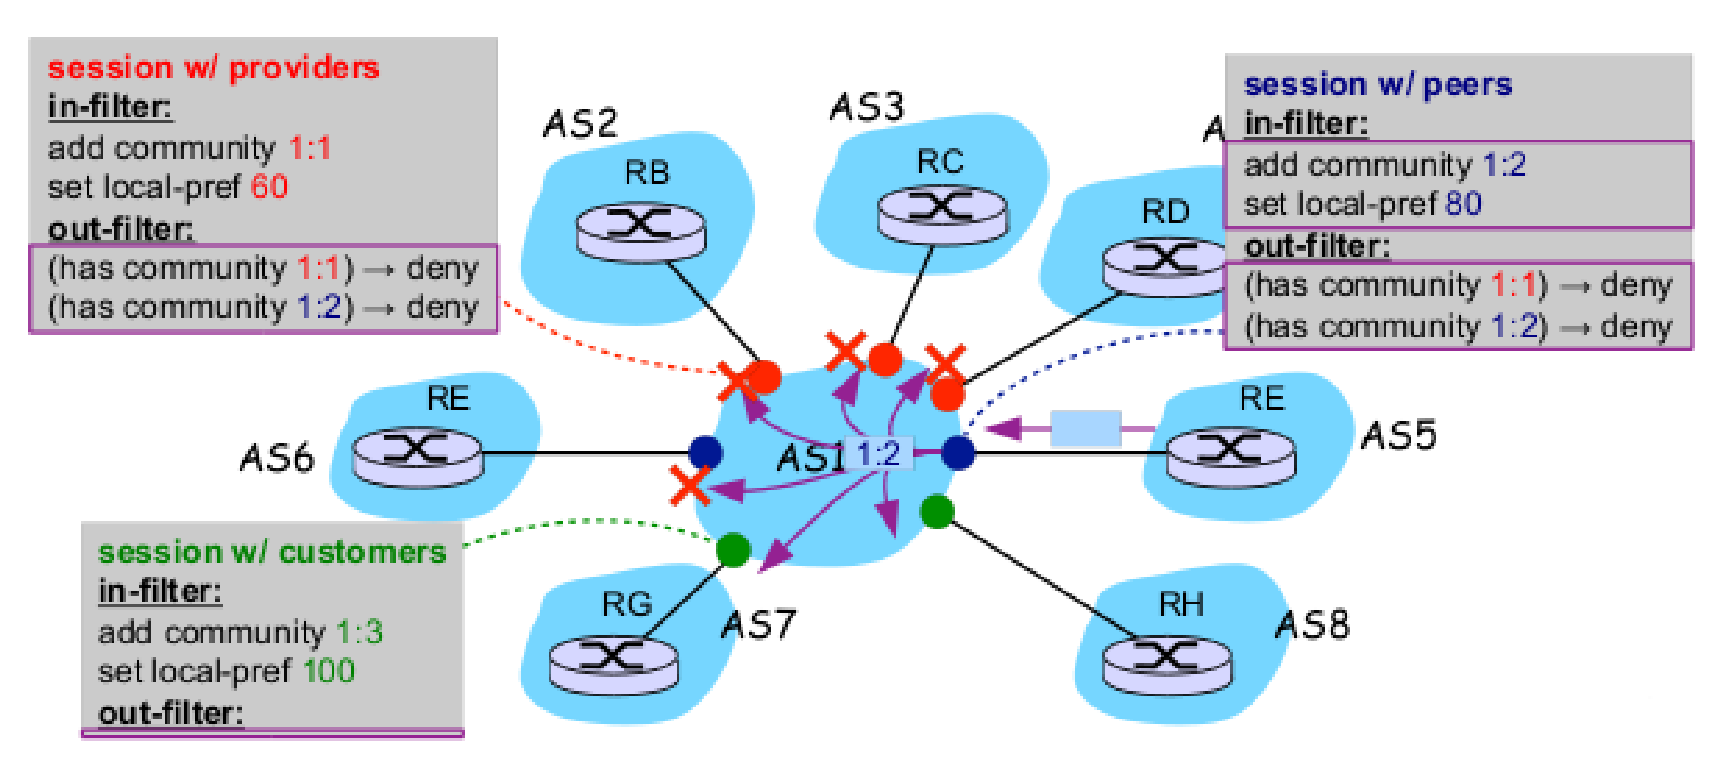
\includegraphics[width=\textwidth]{communities.eps}

\paragraph{Exemple plus complexe: ISP de recherche fournissant 2 types de
  services}

Les universités ont accès au réseau de recherche, les universités et
les institutions gouvernementales ont accès à l'internet commercial.

Pour mettre cela en place, il suffit de ``tagger'' les routes (avec
des communautés) apprises depuis des destinations de recherche ou
commerciales. Ensuite il ne faut annoncer que les universités qu'au
réseau de recherche et le réseau de recherche qu'aux universités.

\paragraph{ISP commercial fournissant 2 services de transit}

Le transit ``plein'' (annoncer toutes les routes connues aux clients,
et les routes des clients aux autres clients, aux pairs et aux
fournisseurs) et des routes clientes uniquement (n'annoncer à ces
clients que les routes apprises par d'autres clients, n'annoncer les
routes apprises par ce client qu'aux autres clients)

\paragraph{Autres utilisations}

On peut utiliser les communautés pour tagger la provenance des routes
(pays), le point d'interconnexion d'où a été reçue la route, etc.

Une fois que les communautés sont apposées sur les routes, on peut les
utiliser comme bon nous semble, par exemple faire des annonces
sélectives sur bases des communautés, de l'AS-PATH prepending, etc.

\paragraph{Inconvénients}

Les communautés sont un attribut transitif. Dans certains cas c'est un
atout, différents AS peuvent ainsi collaborer, mais en général ça
donne surtout des routes polluées par un nombre parfois impressionnant
de communautés, inutiles, mais les routeurs doivent quand même
regarder ces communautés (consommation, mémoire, ...) et générallement
les communautés ont une sémantique locale uniquement.

La meilleure chose à faire pour un routeur qui utilise les
communautés, c'est de s'assurer que ces dernières ne sont pas
annoncées inutilement à l'ensemble de l'internet.

\section{Stabilité}

\subsection{Nombre de messages échangés}

Bien que BGP soit un protocole incrémental, il n'en reste pas moins
très bavard, pour plusieurs raisons:

\begin{itemize}
\item Les réseaux apparaissent et disparaissent
\item Il y a toujours un routeur qui redémarre quelque part
\item Disfonctionnements matériels, lignes arrachées, carte réseau qui
  ``flappe'', ...
\item Mauvaise configuration
\item Exploration du chemin (plusieurs itérations nécessaires avant de
  trouver la meilleure route)
\item Bugs logiciels
\item Instabilité IGP exportée à l'extérieur de l'AS (tie-break IGP et
  règle ``NEXT-HOP le plus proche feront qu'un routeur pourrait
  changer de meilleure route sans arrêt)
\item Algorithmes de routage secrets tentant des astuces suspectes ...
\item Interactions politiques louches
\item Gnomes, étincelles, fées, etc.
\end{itemize}

\paragraph{Comment réduire le nombre de messages UPDATE ?}

Le MRAI (Minimum Route Advertisement Interval) peut être augmenté
(réduit le nombre de messages mais peut allonger le temps de
convergence de BGP)

La plupart des routes ne changent pas fréquemment, une petite part des
routes sont responsables de la plupart des messages BGP échangés. On
peut associer un compteur pénalisant à chaque route, l'incrémenter
chaque fois qu'une route change et utiliser un délai exponentiel pour
lentement diminuer le compteur sur la durée.

Les routes avec un compteur trop élevé sont alors simplement
supprimées pour un certain temps.

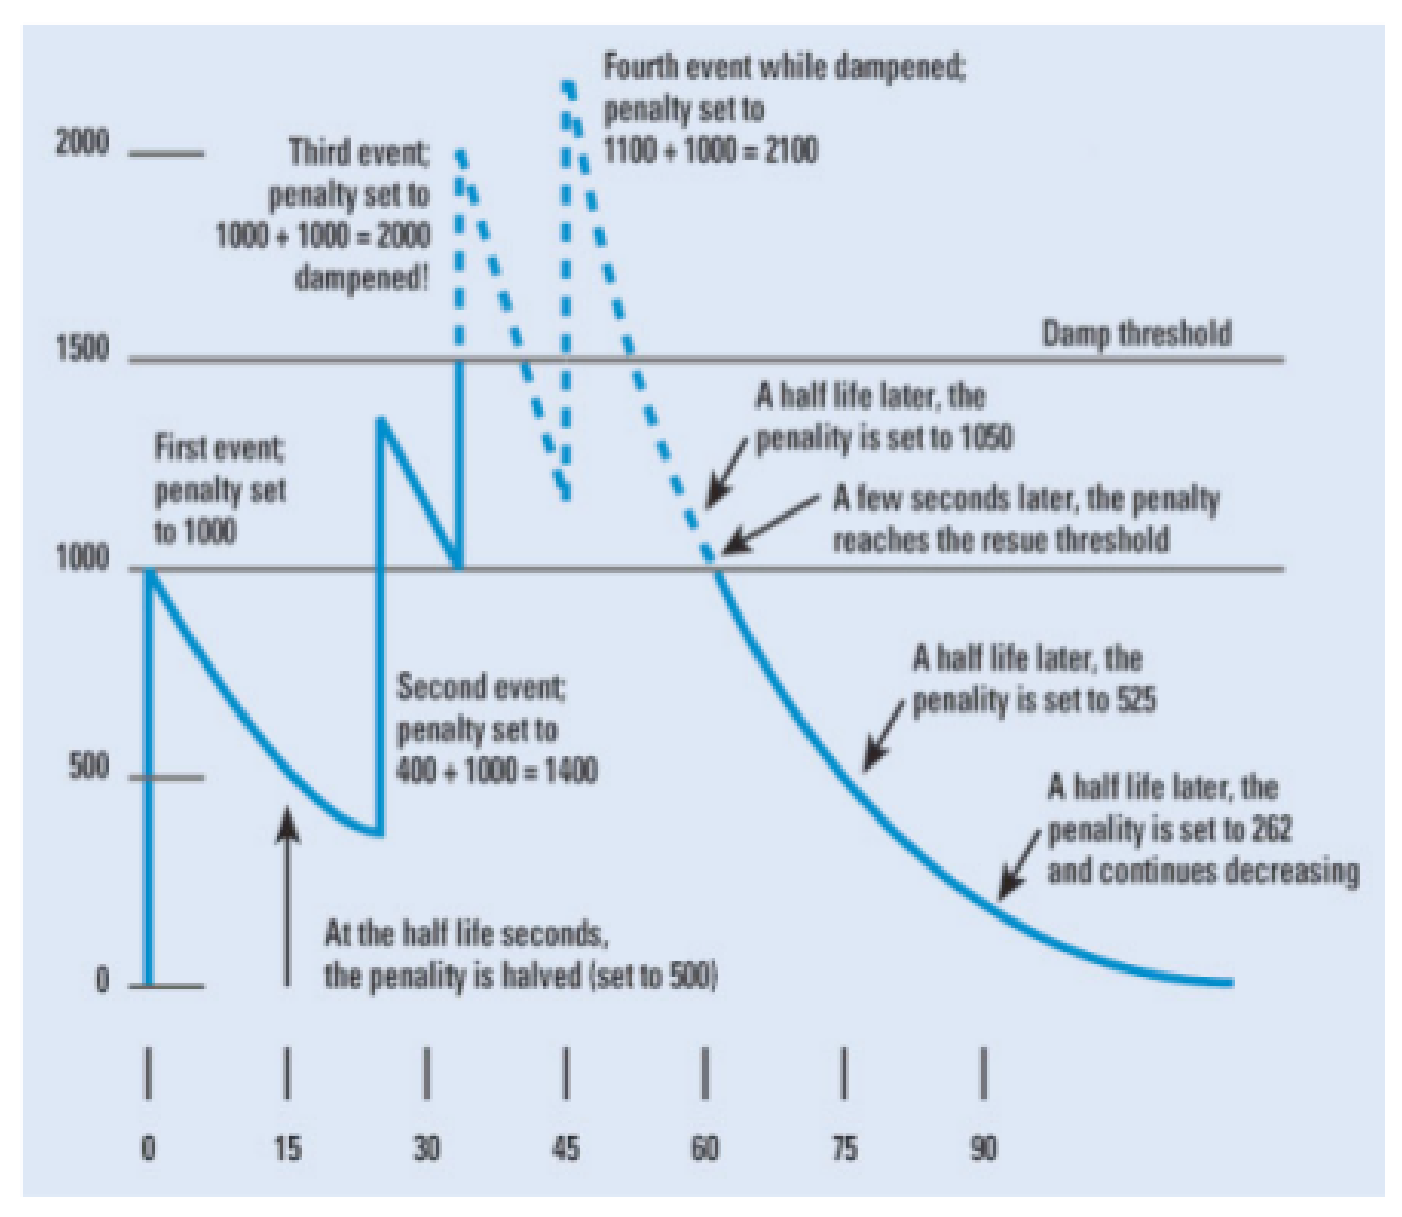
\includegraphics[width=\textwidth]{bgpdampening.eps}

L'utilisation de cette technique (BGP dampening) est découragée
aujourd'hui, car elle peut avoir un effet néfaste en diminuant la
convergence pour des préfixes valides mais qui doivent faire une
exploration du chemin avant de trouver leur meilleure valeur.

\subsubsection{Stable Path Problem (SPP)}

Raisonner quant à la conformité d'un système BGP est un problème
toujours ouvert aujourd'hui.

Le système a-t-il une solution ? Combien de temps durera la
convergence ?

Le SPP est une première tentative pour formaliser la manière dont BGP
fonctionne.

Un SPP est composé d'un graphe $G=(V, E)$, $V = \{0,1,2,\dots\}$,
$peers(u)=\{w|\{u,w\} \in E\}$, par convention, $0$ est le noeud
origine.

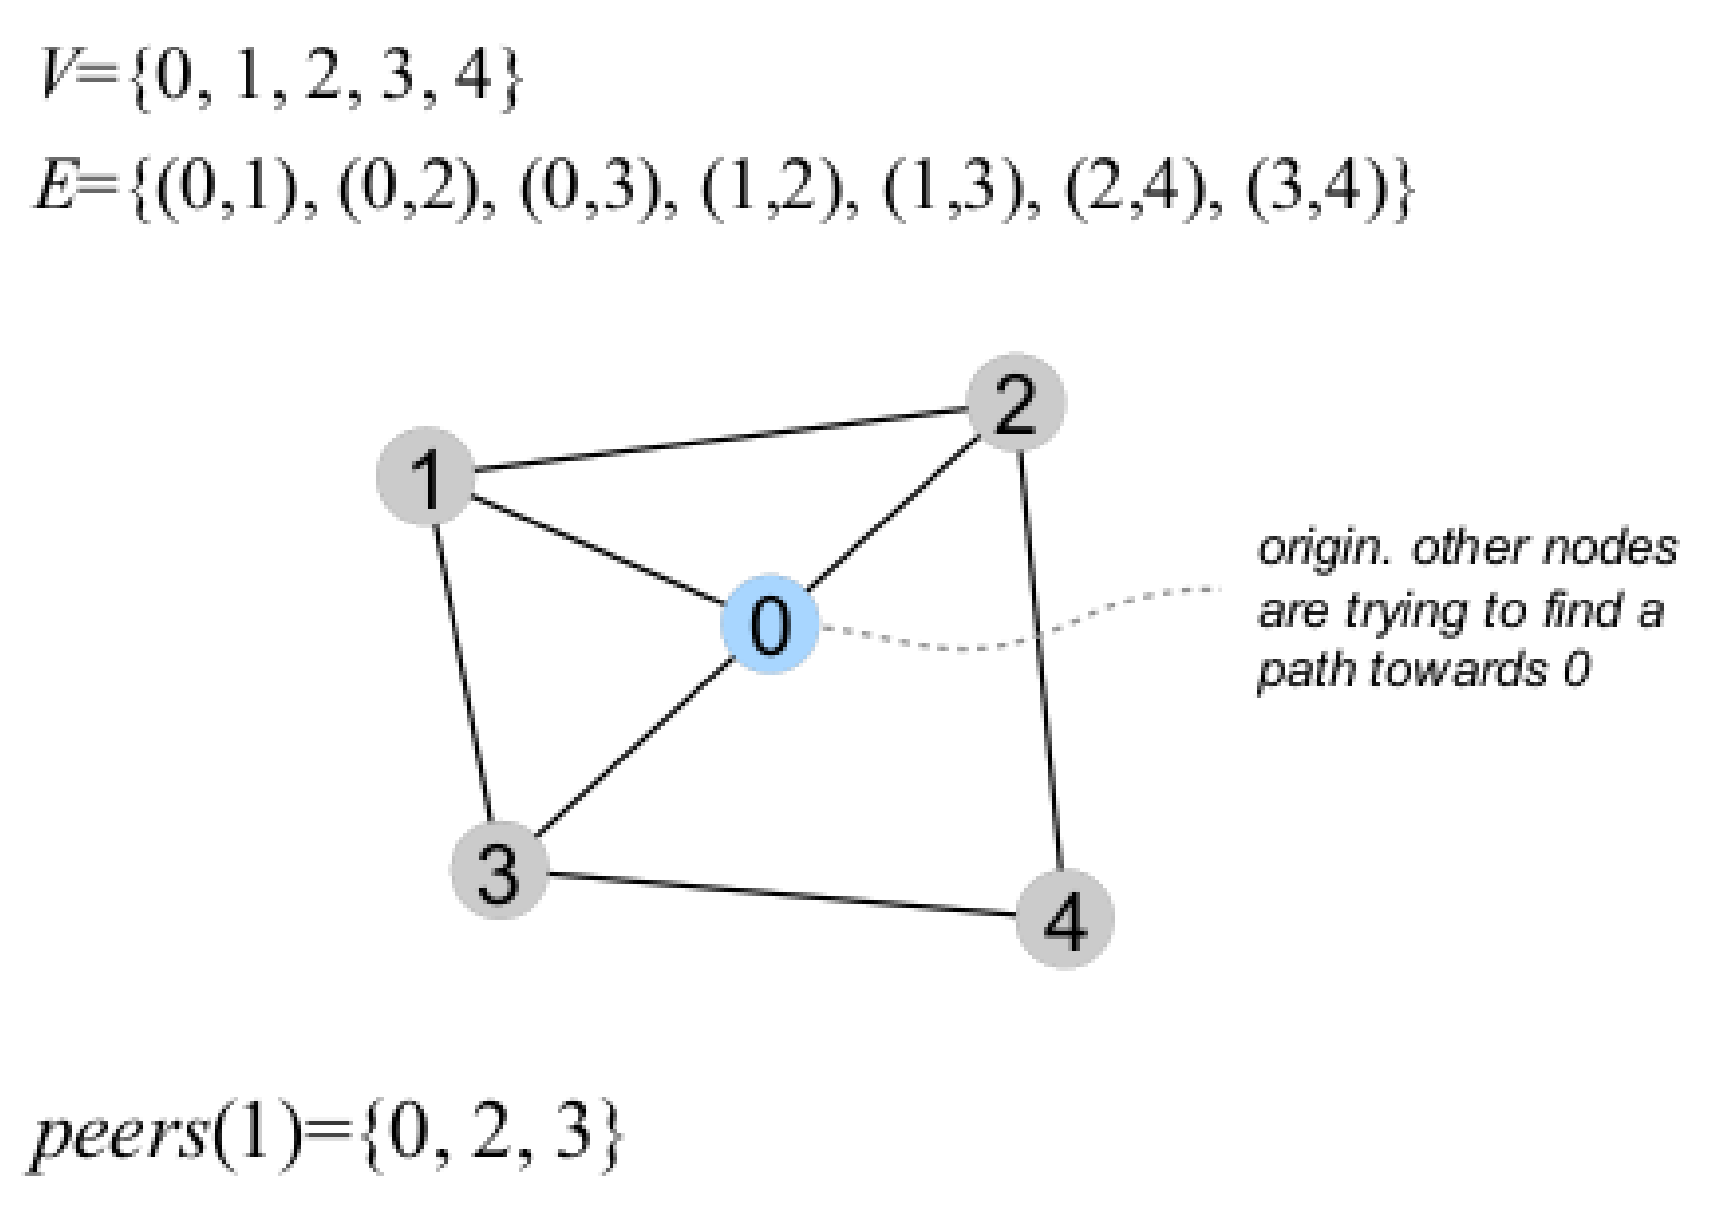
\includegraphics[width=\textwidth]{sppex1.eps}

Un chemin est une séquence $v_k, v_{k-1}, \dots, v_0$de noeuds telle
que chaque paire successive dans la séquence forme un arc dee $V$. Le
chemin vide est désigné par $\epsilon$. Chaque chemin non vide a une
direction de son premier noeud $v_k$ vers son dernier noeud $v_0$.

Pour chaque noeud $v$, $P^v$ désigne l'ensemble des chemins permis de
$v$ à $0$.

Si $P = (v, v_k, \dots, v_0) \in P^v$ , $v_k$ est appelé NEXT-HOP du
chemin $P$.

$P^*$ est l'union de tous les $P^v$

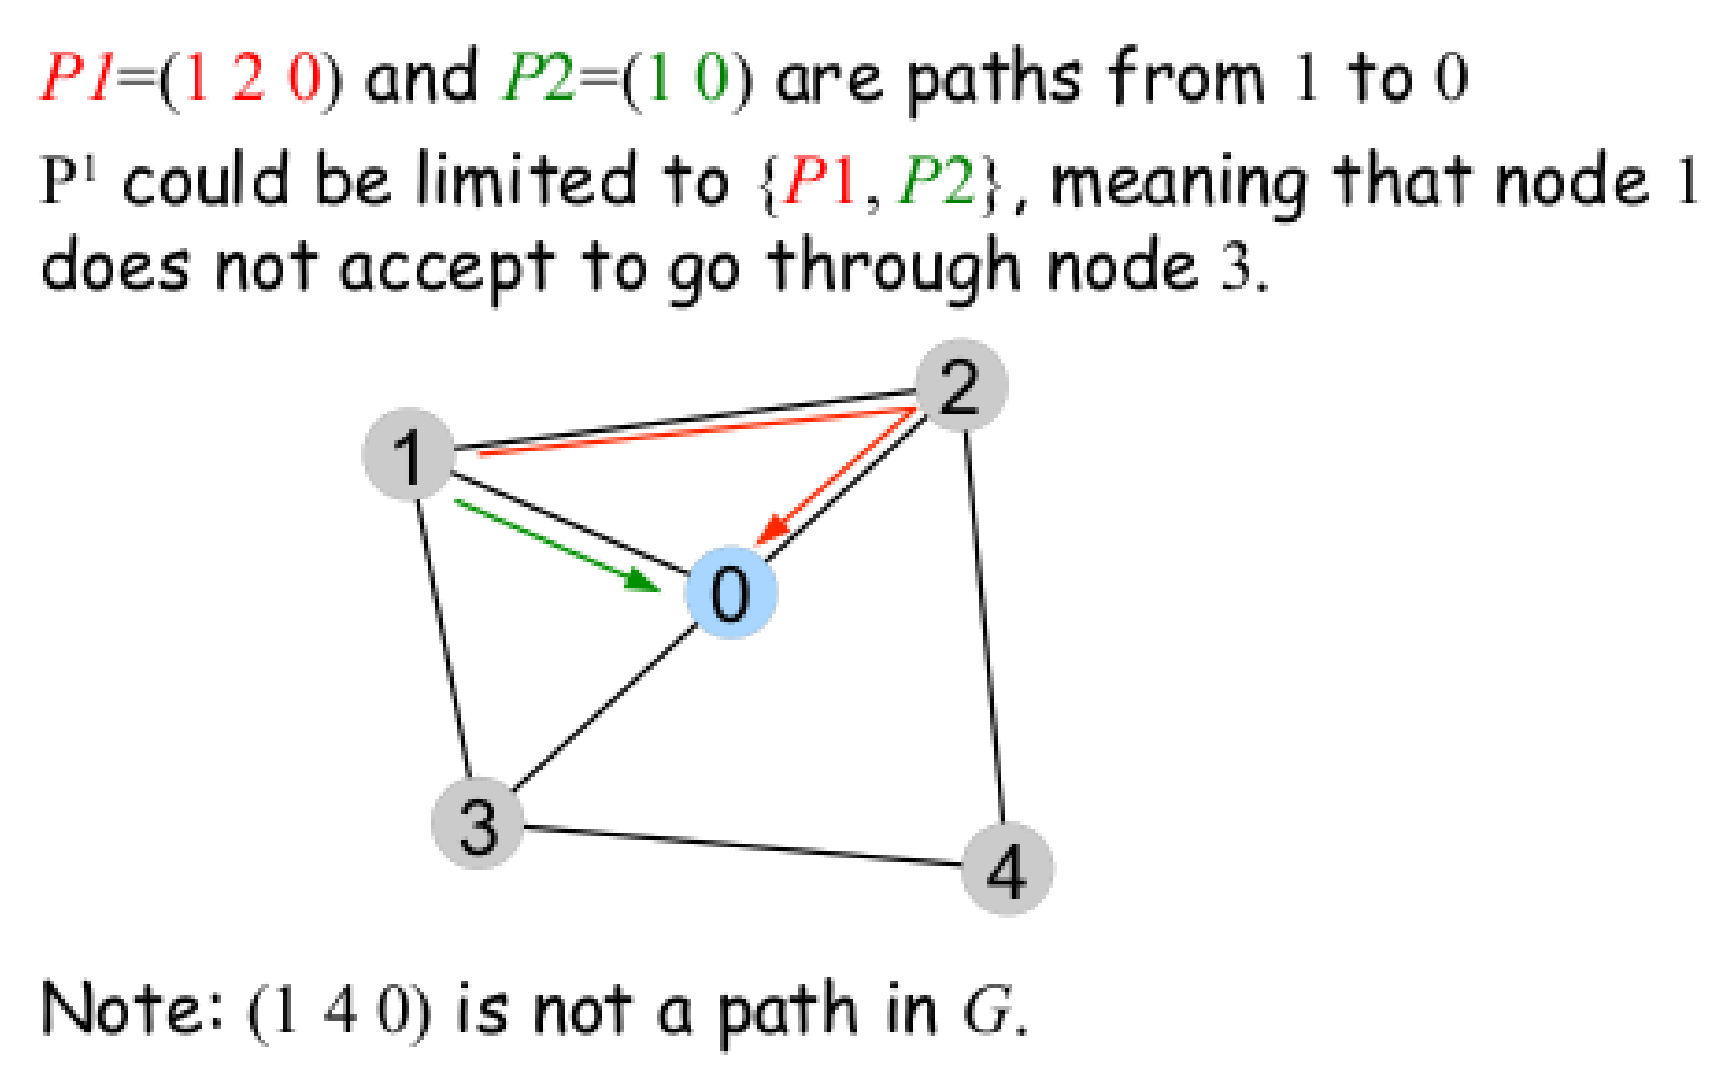
\includegraphics[width=\textwidth]{sppex2.eps}

Le rang d'un chemin pour un noeud $v$ est une fonction $\lambda^v :
P^v \rightarrow R^+$ qui represente comment $v$ range ses chemins
permis.

Si $P1, P2, P^v$ et $\lambda^v(P1) < \lambda^v(P2)$, alors $P2$ est
dit préféré à $P1$.

$\Lambda = \{\lambda^v | v \in V-\{0\}\}$

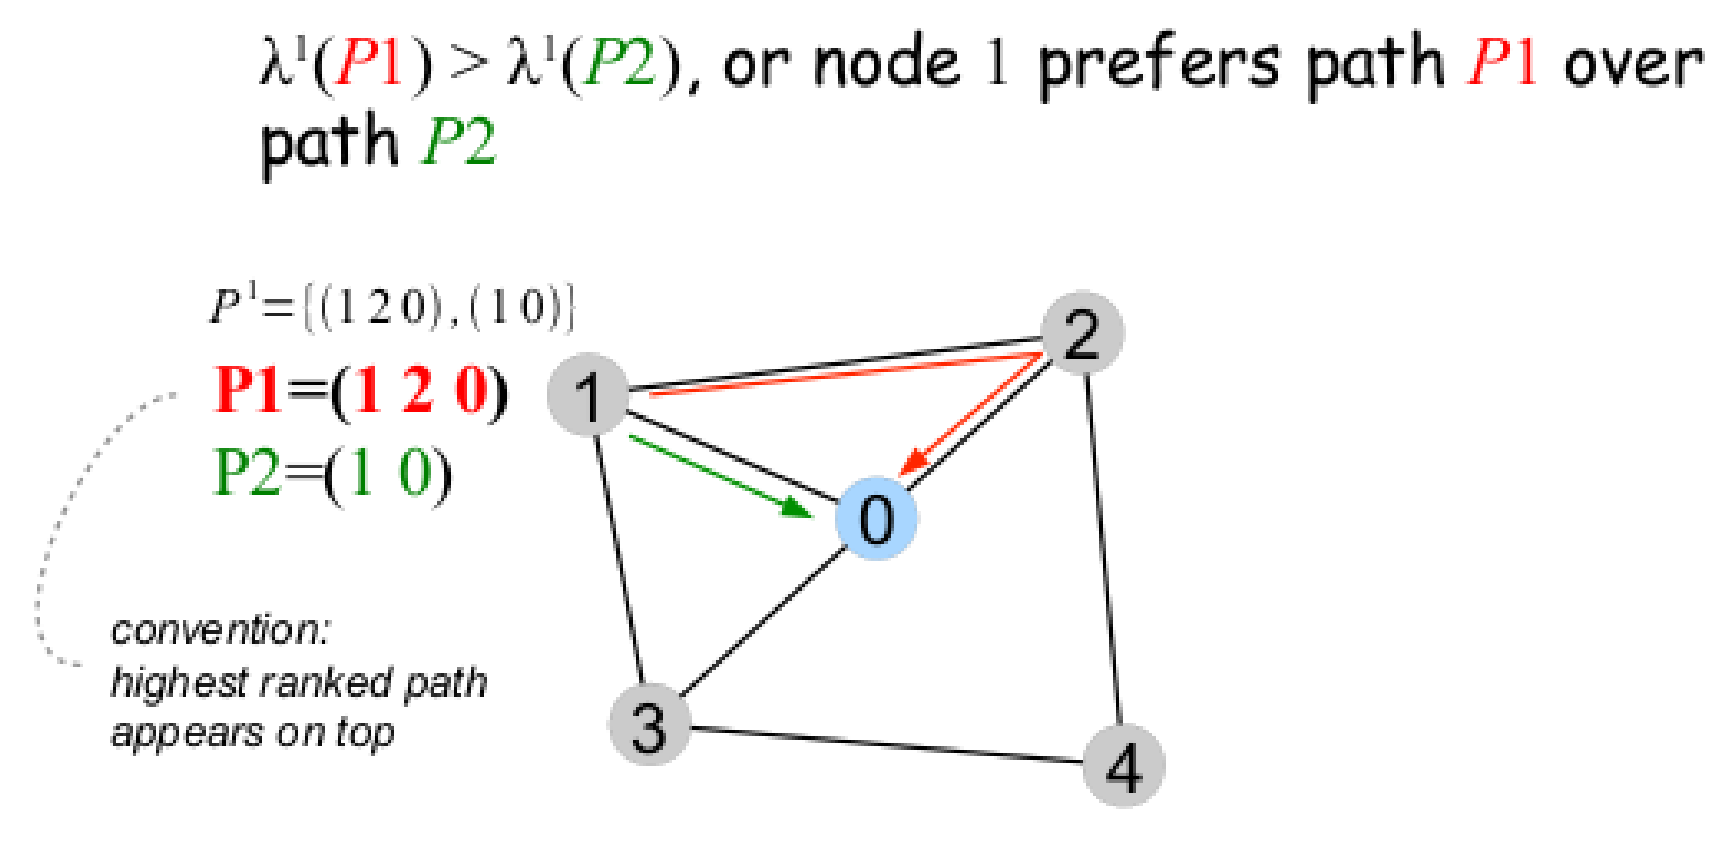
\includegraphics[width=\textwidth]{sppex3.eps}

Une instance SPP $S = (G, P^*, \Lambda)$ admet $P^0=\{(0)\}$.

$\pi(v)$ représente une assigation de chemin pour $v$. Si la valeur
est $\epsilon$, on considère qu'aucun chemin ne lie $v$ à $0$ dans
l'assignation courante.

$choices(\pi, v)$ représente les chemins possibles, via l'assignation
courante, que $v$ a pour atteindre $0$.

Le meilleur chemin P dans l'ensemble $W$ pour un noeud $u$, noté
$best(W, u)$ est tel que $\lambda^u(P)$ est plus grand que tout autre
chemin de $W$.

Une assignation $\pi$ est stable en $u$ si $\pi(u) = best(choices(\pi,
u), u)$ qui signifie que $u$ est assigné au meilleur de ses choix.

Une assignation est stable si elle est stable en chacun de ses noeuds.

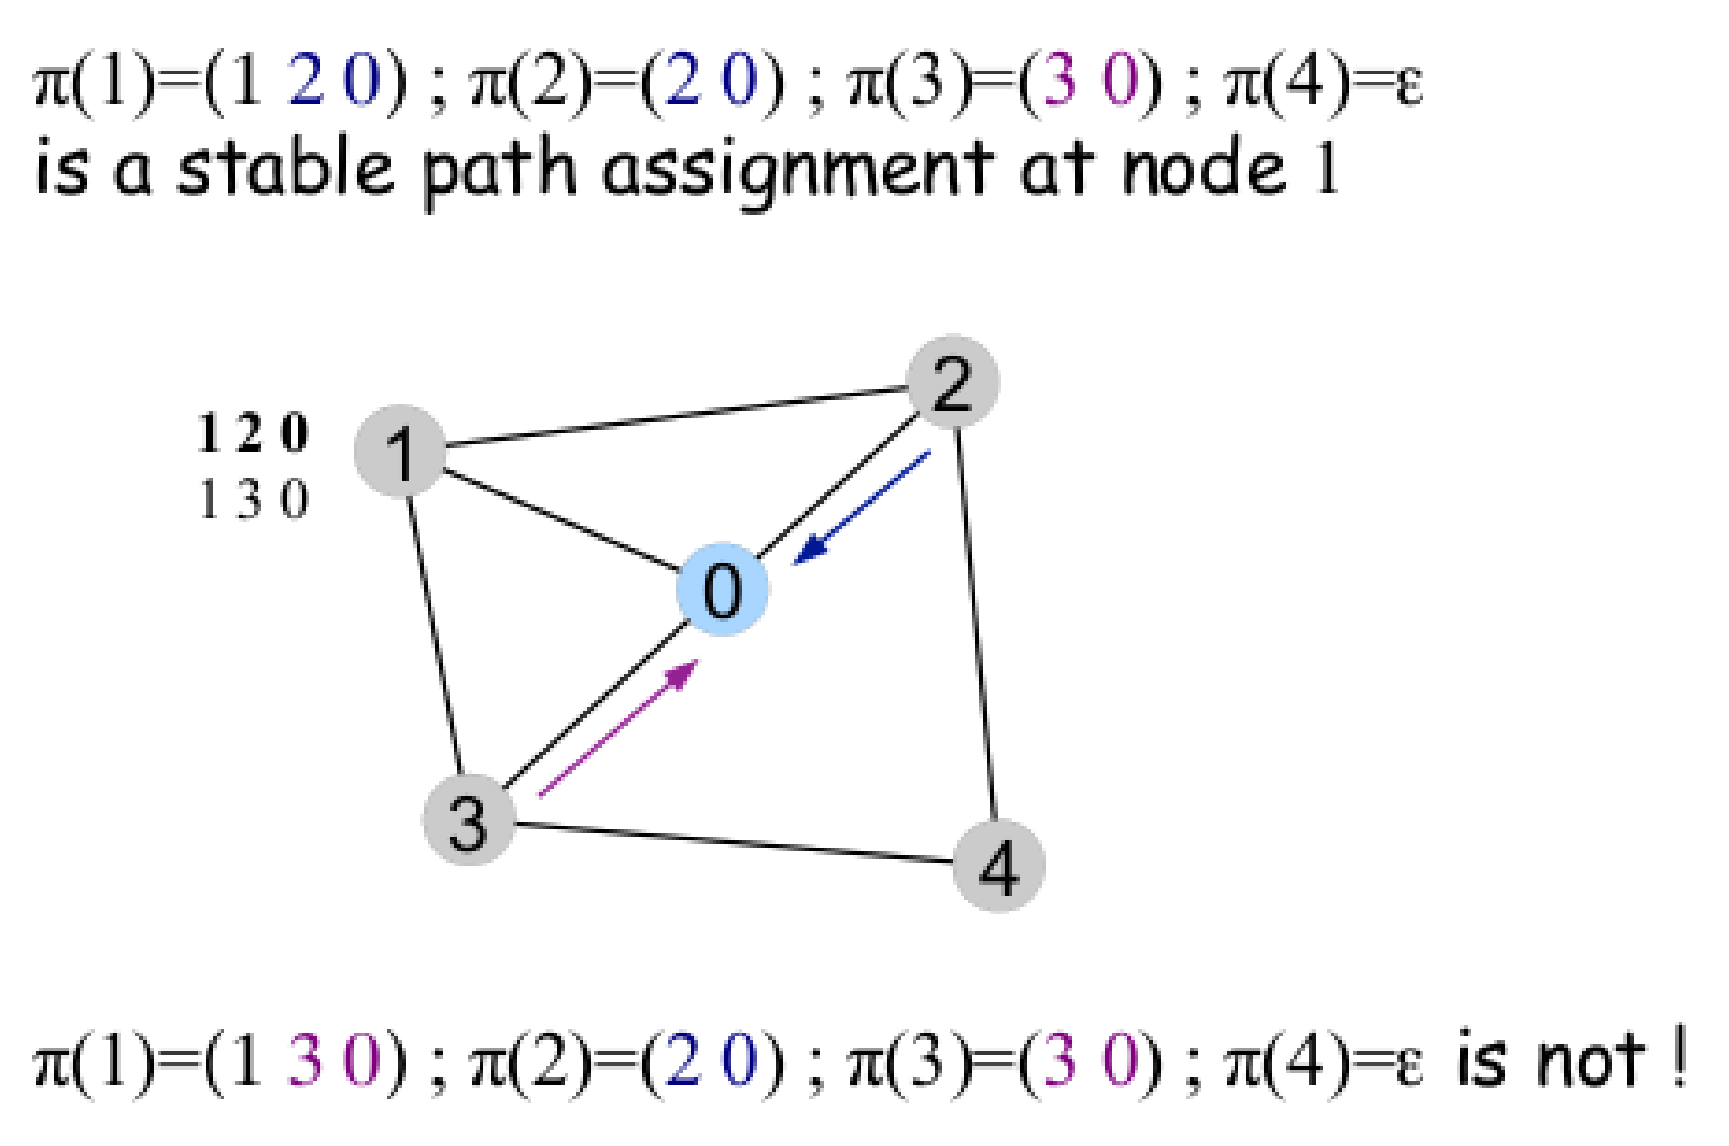
\includegraphics[width=\textwidth]{sppex4.eps}

Une instance SPP est solvable si une assignation stable existe pour
l'intance, on appelle cette assignation la solution de l'instance;
sinon l'instance est dite insolvable.

Une méthode pour trouver les assignements possibles, ainsi que les
solutions, est de faire un tri topologique sur le graphe de
dépendances, et ensuite d'ajouter les noeuds, dans cet ordre, jusqu'à
ce que tous les noeuds soient ajoutés, on voit alors toutes les
possibilités, pour choisir celles qui sont des solutions, il suffit de
regarder qu'à chaque noeud de l'arbre ainsi construit, la branche est
bien le meilleur choix.

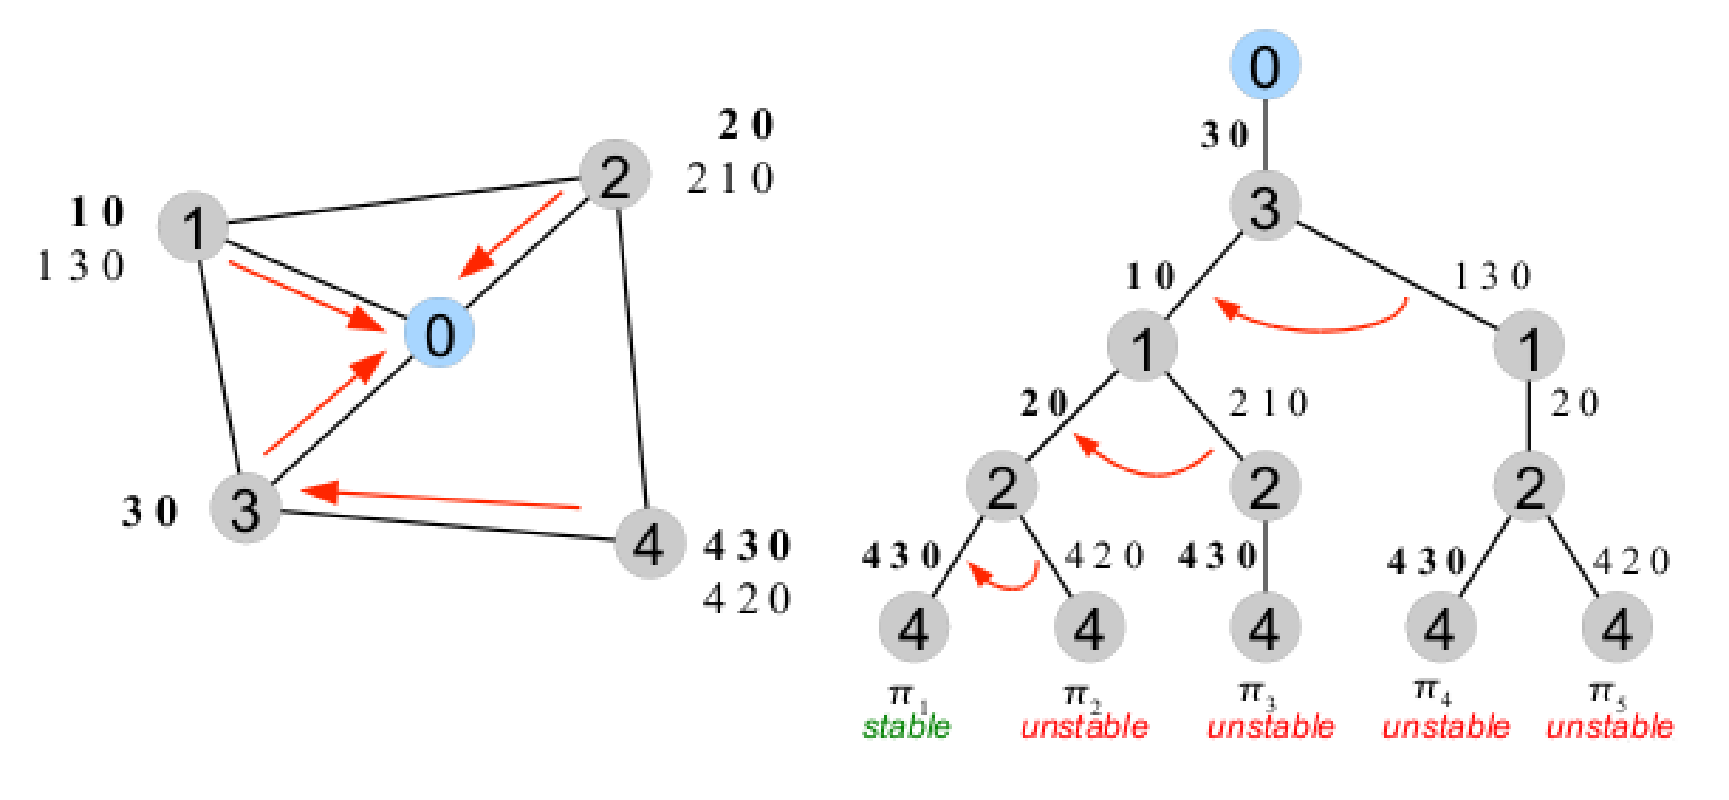
\includegraphics[width=\textwidth]{sppex5.eps}

Dans cet exemple, la solution est un shortest-path tree, ce n'est pas
toujours le cas. Cette méthode se base sur le fait que le graphe de
dépendances est un DAG, ce n'est pas une condition nécessaire pour que
l'instance ait une solution. (Exemple: DISAGREE, dont le graphe de
dépendances est ci-dessous)

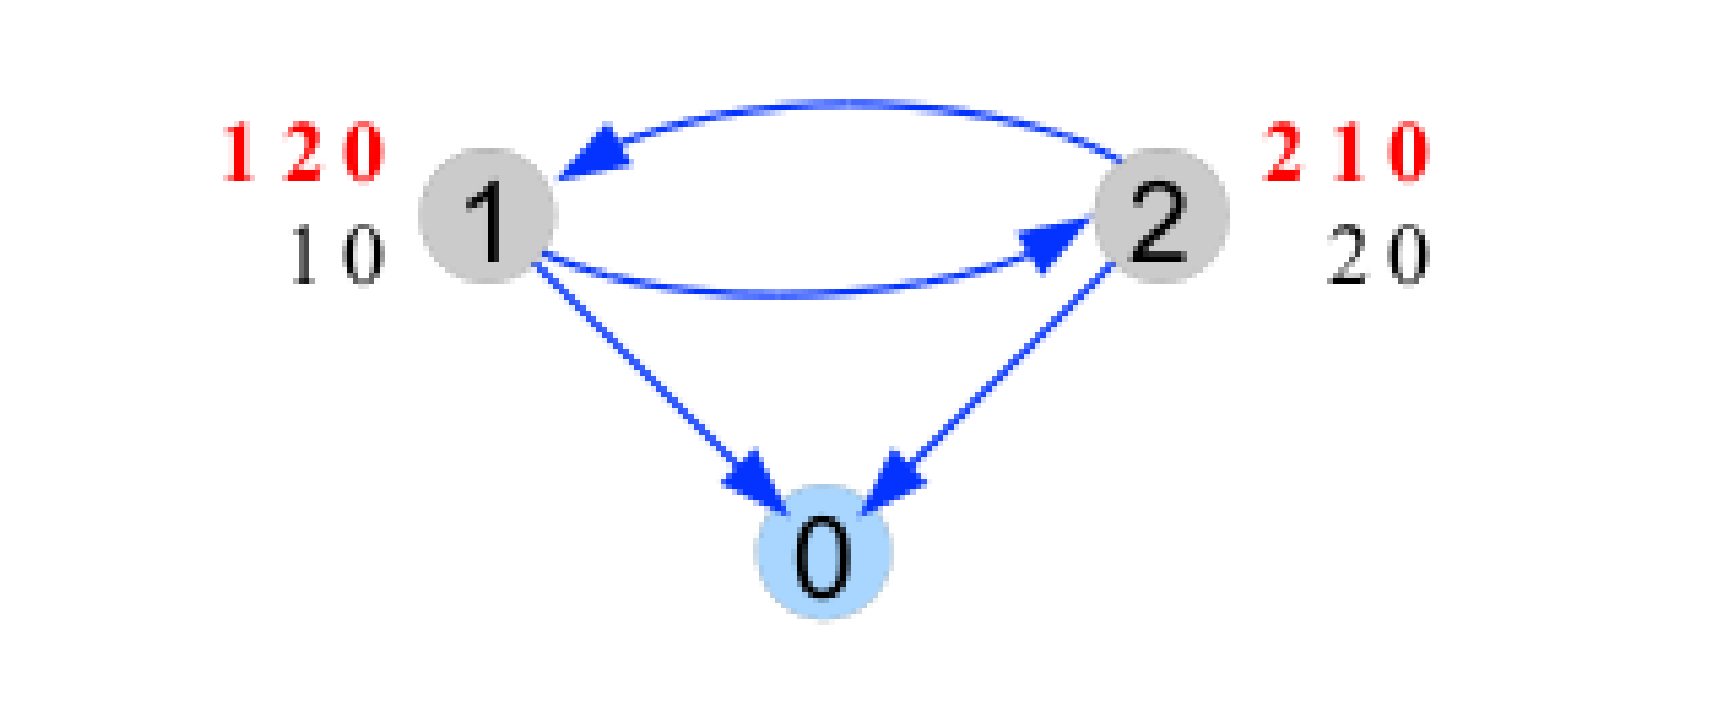
\includegraphics[width=0.5\textwidth]{sppex6.eps}

\paragraph{Séquence d'activation}

Considérons maintenant le même modèle légèrement modifié, c'est-à-dire
que chaque noeud est indépendant et voit une partie limitée du
réseau. À chaque nouveau ``temps'', un noeud reçoit l'information d'un
voisin, la traite et choisit une nouvelle meilleure route. L'ordre
dans lequel les noeud s'activent est la séquence d'activation.

Exemple de séquence d'activation avec DISAGREE:

\begin{tabular}{|c|c|c|c|}
  \hline
  Step & Event & Noeud 1 & Noeud 2 \\
  \hline
  0 & $(0, 1): \pi(0) = (0)$ & choices=\{(1 0)\} & \\
  & & best=(1 0) & \\
  \hline
  1 & $(1, 2): \pi(1) = (1 0)$ & & choices=\{(2 1 0)\} \\
  & & & best=(2 1 0) \\
  \hline
  2 & $(0, 2): \pi(0) = (0)$ & & choices=\{(2 1 0), (2 0)\} \\
  & & & best=(2 1 0) \\
  \hline
  3 & $(2, 1): \pi(2) = (2 1 0)$ & choices=\{(1 0)\} & \\
  & & best=(1 0) & \\
  \hline
\end{tabular}

On obtient dans ce cas une assignation stable, voici un autre exemple
où les choses se passent moins bien:

\begin{tabular}{|c|c|c|c|}
  \hline
  0 & $(0, 1): \pi(0) = (0)$ & choices=\{(1 0)\} & \\
  & & best=(1 0) & \\
  \hline
  1 & $(0, 2): \pi(0) = (0)$ & & choices=\{(2 0)\} \\
  & & & best=(2 0) \\
  \hline
  2 & $(1, 2): \pi(1) = (1\ 0)$ & & choices=\{(2 0), (2 1 0)\} \\
  & & & best=(2 1 0) \\
  \hline
  3 & $(2, 1): \pi(2) = (2\ 0)$ & choices=\{(1 0), (1 2 0)\} & \\
  & & best=(1 2 0) & \\
  \hline
  4 & $(2, 1): \pi(2) = (2\ 1\ 0)$ & choices=\{(1 0)\} & \\
  & & best=(1 0) & \\
  \hline
  5 & $(1, 2): \pi(1) = (1\ 2\ 0)$ & & choices=\{(2 0)\} \\
  & & & best=(2 0) \\
  \hline
  6 & $(1, 2): \pi(1) = (1\ 0)$ & & choices=\{(2 0), (2 1 0)\} \\
  & & & best=(2 1 0) \\
  \hline
  7 & $(2, 1): \pi(2) = (2\ 0)$ & choices=\{(1 0), (1 2 0)\} & \\
  & & best=(1 2 0) & \\
  \hline
  ... & ... & ... & ... \\
\end{tabular}

\paragraph{Exemple d'instance de SPP insolvable}

Voici un exemple de séquence d'activation, on aboutira en fait
toujours à un cycle (on considère ici que chaque noeud fait une action
en même temps en reçoit les infos des autres noeuds en même temps).

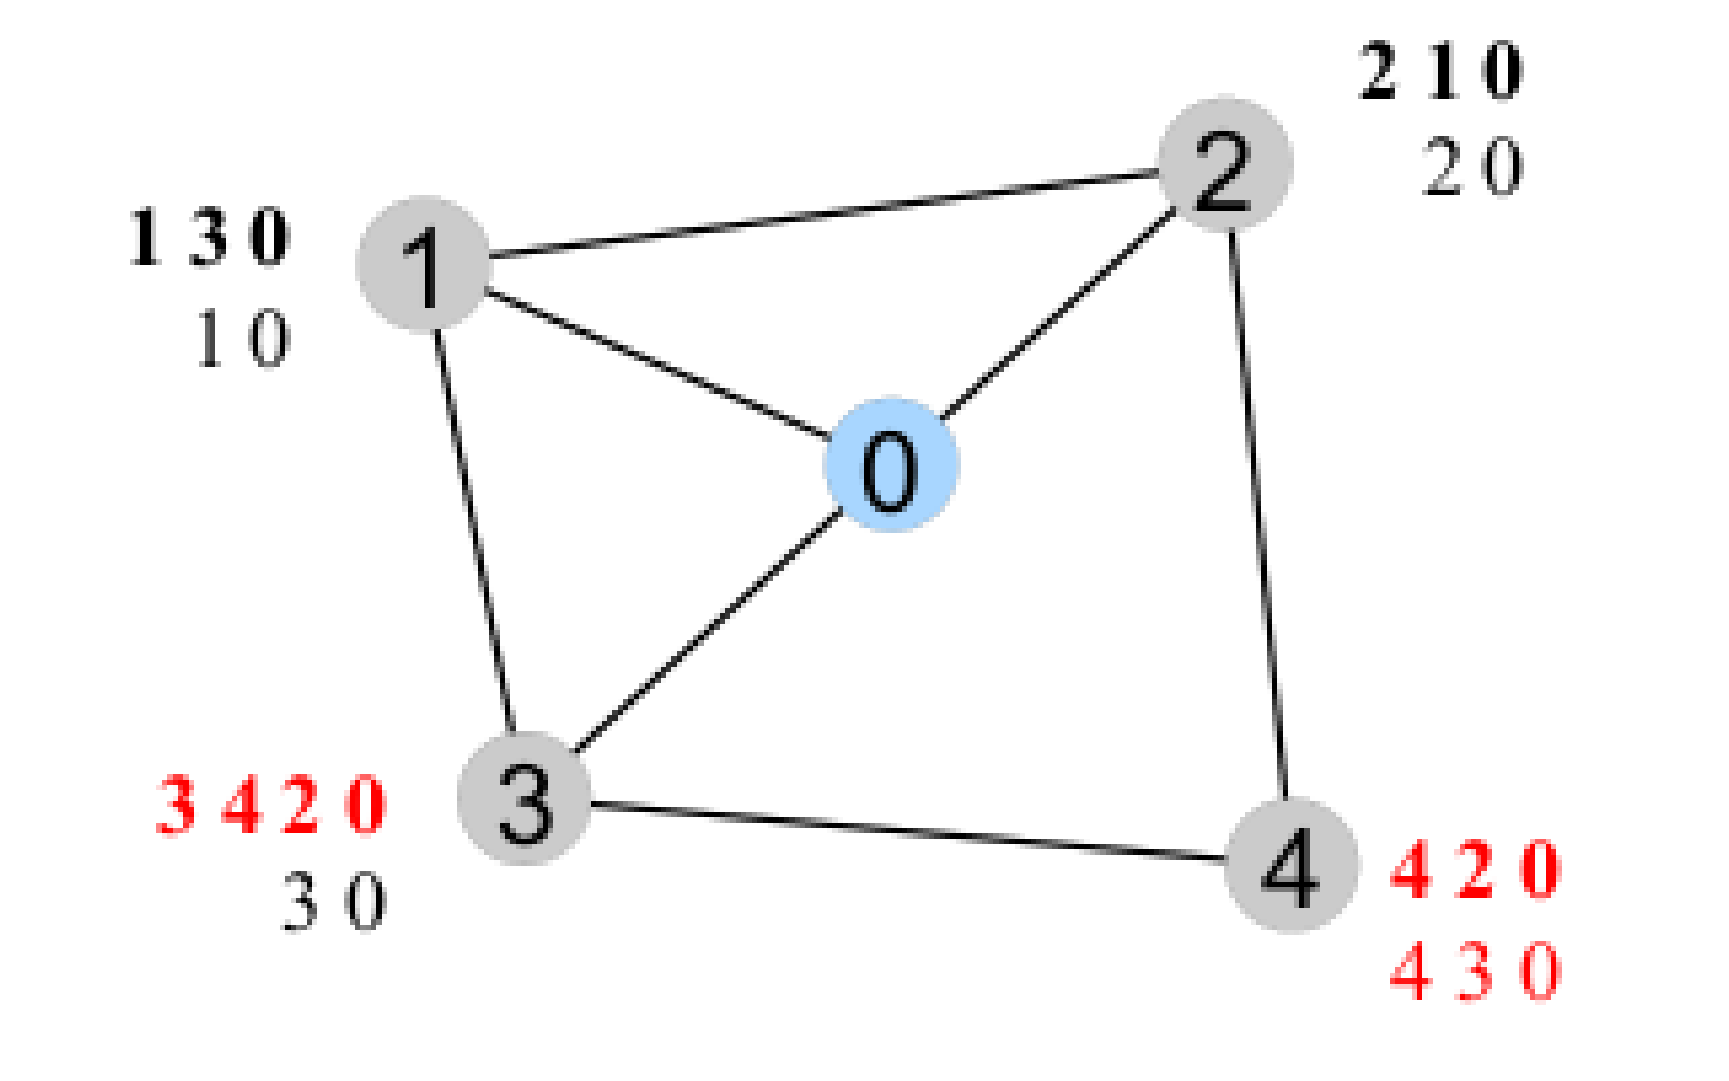
\includegraphics[width=0.5\textwidth]{sppex7.eps}

\begin{tabular}{|c|c|c|c|c|}
  \hline
  Pas & Noeud 1 & Noeud 2 & Noeud 3 & Noeud 4 \\
  \hline
  0 & (1 0) & (2 0) & (3 0) & \\
  & (1 0) & (2 0) & (3 0) & \\
  \hline
  1 & (1 0), (1 3 0) & (2 0), (2 1 0) & & (4 2 0), (4 3 0) \\
  & (1 3 0) & (2 1 0) & & (4 2 0) \\
  \hline
  2 & & (2 0) & (3 0), (3 4 2 0) & (4 3 0) \\
  & & (2 0) & (3 4 2 0) & (4 3 0) \\
  \hline
  3 & (1 0) & & (3 0) & (4 2 0) \\
  & (1 0) & & (3 0) & (4 2 0) \\
  \hline
  4 & (1 0), (1 3 0) & (2 0), (2 1 0) & (3 0), (3 4 2 0) & (4 2 0), (4 3 0) \\
  & (1 3 0) & (2 1 0) & (3 4 2 0) & (4 2 0) \\
  \hline
  5 & (1 0) & (2 0) & & $\emptyset$ \\
  & (1 0) & (2 0) & & $\epsilon$ \\
  \hline
  6 & & (2 0), (2 1 0) & (3 0) & (4 2 0) \\
  & & (2 1 0) & (3 0) & (4 2 0) \\
  \hline
  7 & (1 0), (1 3 0) & & (3 0), (3 4 2 0) & (4 3 0) \\
  & (1 3 0) & & (3 4 2 0) & (4 3 0) \\
  \hline
  8 & (1 0) & (2 0) & (3 0) & $\emptyset$ \\
  & (1 0) & (2 0) & (3 0) & $\epsilon$ \\
  \hline
  ... & ... & ... & ... & ...
\end{tabular}

Mauvaise nouvelle: la solvabilité est NP-complète, malgré ce résultat,
des choses intéressantes peuvent malgré tout être dites.

Par exemple, ce n'est pas parce qu'un système est solvable qu'il
convergera forcément. Une instance SPP est sûre si elle est solvable
sous n'importe quelle séquence d'activation où aucune information
n'est perdue.

\paragraph{Roues de dispute}

On peut voir DISAGREE comme une roue de dispute à deux rayons.

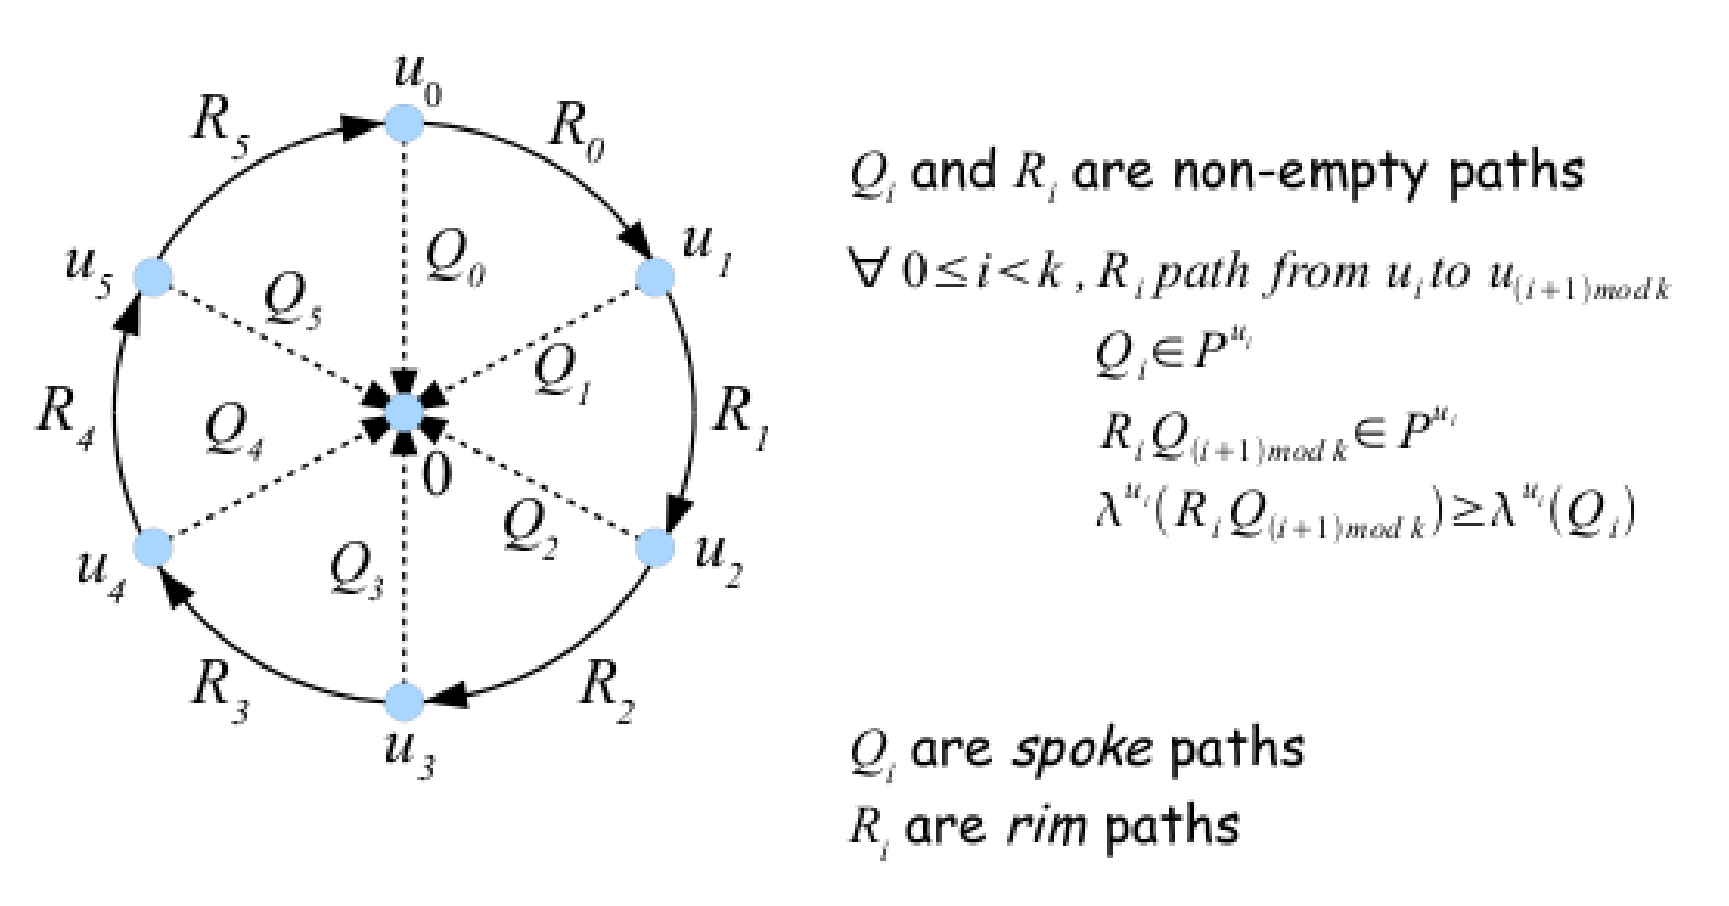
\includegraphics[width=\textwidth]{disputewheel.eps}

Théorèmes: Si une instance SPP n'a pas de roue de dispute, alors elle
est solvable, a une solution unique et est sûre.

\paragraph{Limitations}

Le formalisme SPP est difficile à appliquer directement à un système
BGP car les fonctions de rang ne sont pas explicites dans les filtres
de routage BGP.

Le condition ``Pas de roue de dispute'' est trop forte dans certains
cas.

Les politiques de routage ne sont toujours pas bien comprises et font
l'objet de beaucoup de recherches.

Toutefois, des études ont prouvé que si chaque AS suit les deux lignes
directrices suivantes, alors le système serait sûr:

\begin{itemize}
\item Ranger les routes de telle sorte que celles des clients soient
  préférées à celles des pairs, qui elles-mêmes doivent être préférées
  à celles des fournisseurs.
\item Filtrer les routes pour que les chemins entre fournisseurs et/ou
  pairs ne soient pas autorisés.
\end{itemize}

\subsubsection{Problèmes d'iBGP}

\begin{itemize}
\item Les routes peuvent osciller à cause du MED
\item BAD GADGET peut être ``implémenté'' en iBGP
\item On peut créer des boucles de forwarding en iBGP
\end{itemize}

\chapter{IPv6}

\section{Motivations}

Le problème principal à court terme est le manque d'adresses IP, en
particulier de classe B. D'autres problèmes sont la structure complexe
des paquets IPv4, le forwarding qui est complexe à implémenter, la
configuration manuelle nécessaire, le manque de sécurité, de mobilité,
la qualité de service non présente, etc.

Le NAT aurait pû être une solution, mais il apporte également son lot
de problèmes: traversée de NAT compliquée, le principe ``end-to-end''
n'est pas respecté, donne une fausse impression de sécurité, les
intermédiaires peuvent modifier le contenu des paquets, etc.

\section{Architecture d'adressage IPv6}

Les adresses seront 4 fois plus longues (128 bits au lieu de 32)

Elles pourront être de trois types: Unicast (adresses habituelles, une
adresse correspond à une interface), Anycast (plusieurs interfaces
peuvent avoir la même adresse, les paquets à destination de cette
adresse étant envoyés à l'interface ``la plus proche'') et Multicast
(plusieurs interfaces ont la même adresse, les paquets à destination
de cette adresse sont envoyés à toutes les interfaces).

Les adresses sont notées en hexadécimal
(``xxxx:xxxx:xxxx:xxxx:xxxx:xxxx:xxxx:xxxx'', les suites de 0 peuvent
être notées ``::'' (une seule fois maximum par adresse), loopback:
``::1'')

\subsection{Adresses Unicast}

Adresses spéciales: ``::1'' (loopback) et ``::'' (unassigned)

Les adresses sont allouées de manière hiérarchique: $N$ bits pour le
préfixe global de routage (identifie l'ISP responsable de l'adresse),
$M$ bits pour l'identifiant de sous-réseau (sous-réseau ou client de
l'ISP) et $128-N-M$ bits pour l'interface (en général, 64 bits, basés
sur l'adresse MAC)

L'IANA contrôle toutes les adresses IP et délègue l'assignement des
blocs à des Registrars Internet Régionaux (RIR).

Une organisation peut recevoir deux types distincts d'adresses IP:
Provider Independent (PI), générallement allouées à des ISP ou
entreprises très grandes directement par les RIR (/32), ou Provider
Aggregatable (PA), /48 dans le cas général, /64 quand un réseau unique
est requis, /128 quand on sait qu'une et une seule interface
l'utilisera.

\begin{center}
  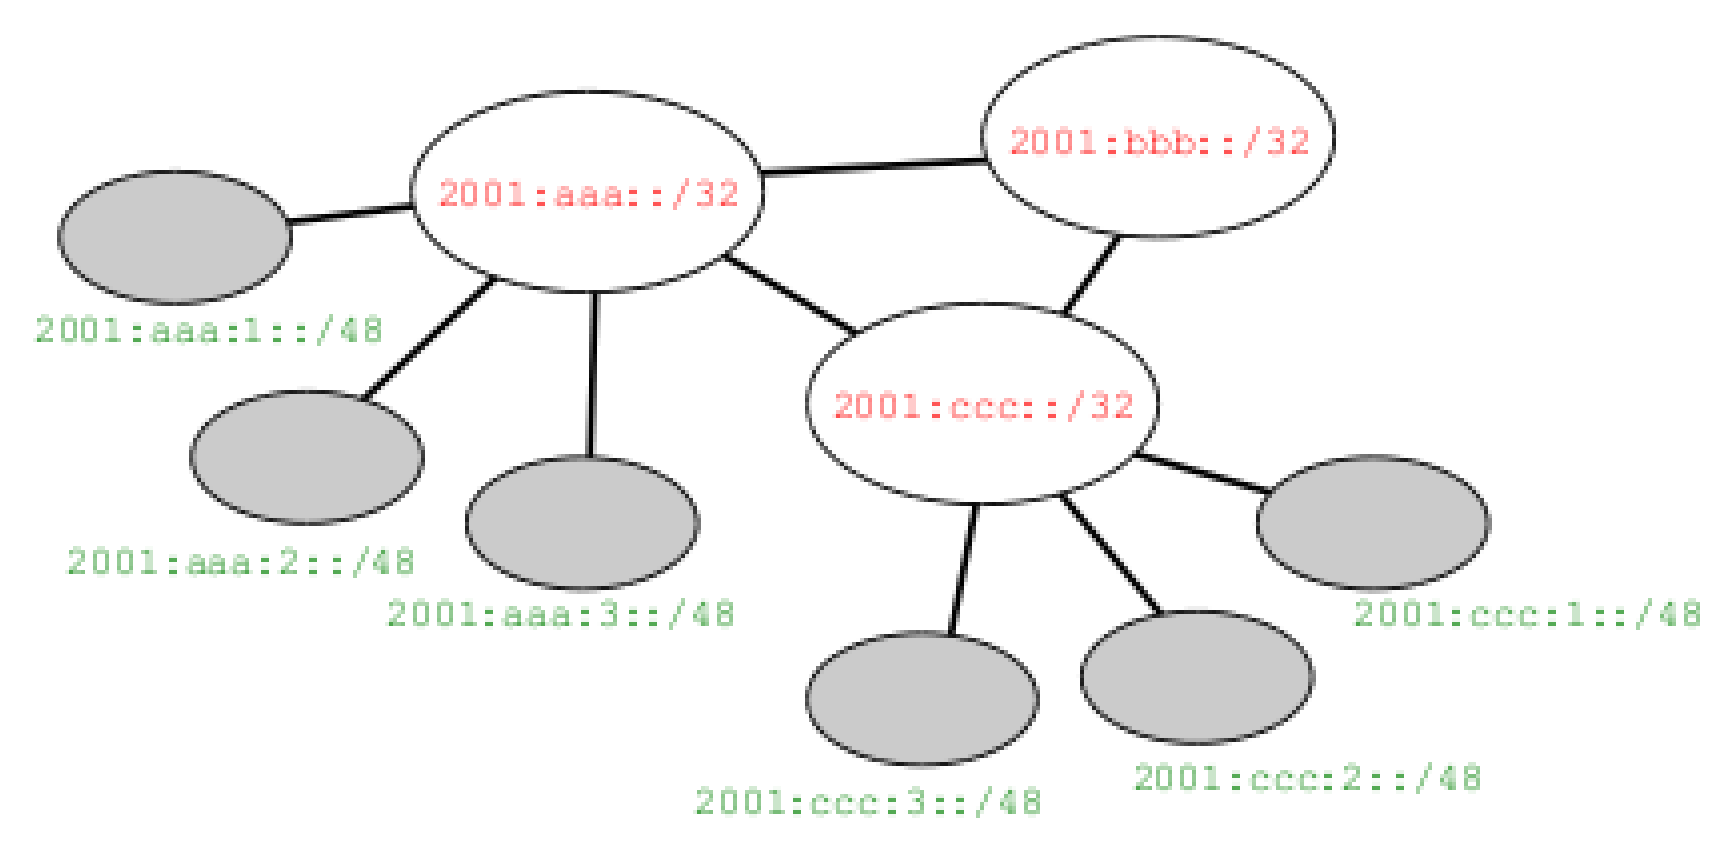
\includegraphics[width=0.75\textwidth]{ipv6allocation.eps}
\end{center}

L'utilisation des adresses PA permet une meilleure aggrégation qu'avec
IPv4 et devrait amener à des tables de routages plus petites.

Un inconvénient est que lorsqu'un client change de provider, il doit
changer les IP de toutes ses interfaces, de plus, un réseau
multi-homed recevra un préfixe différent pour chacun de ses providers,
chaque interface devra alors avoir plusieurs adresses une par préfixe,
la loopback, d'autres adresses ?)

\paragraph{Adresses link-local}

Elles commencent par le préfixe ``FE80:0:0:0'', les 64 bits restants
sont réservés à l'interface; chaque routeur/serveur doit générer une
adresse link-local pour chacune de ses interfaces. Chaque host IPv6
utilisera donc plusieurs adresses IPv6.

\paragraph{Modified EUI-64 format}

L'adresse MAC (EUI-48) est divisée en deux parties au milieu
desquelles on insère la séquence ``FF FE'', on a alors 64 bits (format
EUI-64), le 7è bit est mis à $1$; ce qui donne le modified EUI-64.

\subsection{Adresses Multicast}

Les 8 premiers bits de l'adresse doivent tous être à $1$. le 4
suivants déterminent des flags, les 4 suivants la portée; les 112 bits
restants déterminent l'identifiant du groupe.

Certains groupes sont prédéfinis: tous les systèmes en bordure doivent
appartenir à FF02::1, tous les routeurs à FF02::2, pour la portée
locale, tous les noeuds doivent appartenir à FF02::1, tous les
routeurs à FF02::2, les adresses Solicited-node à FF02::1:FFxx:xxxx où
xx:xxxx sont les 24 bits les moins significatifs de l'adresse IP.

\paragraph{Multicast Ethernet}

Les adresses commençant par 00 sont unicast, par 01 sont multicast et
par FF:FF:FF:FF:FF:FF est l'adresse de broadcasting. Chaque interface
inscrite à un groupe multicast doit écouter l'adresse Ethernet
multicast correspondant à son groupe en plus de son adresse unicast.

\paragraph{Envoyer des paquets IPv6 multicast}

Le préfixe Ethernet 33:33 est réservé pour le multicast IPv6. Pour
envoyer un paquet IPv6 multicast sur Ethernet, un noeud ajoute
simplement les 32 bits de la destination IPv6 après le préfixe 33:33.

\subsection{Adresses Anycast}

On appelle une telle adresse ``Adresse unicast partagée'', elles
servent quand des serveurs multiples redondants proposent le même
service (serveurs DNS par exemple); une telle adresse ressemble à une
adresse unicast mais requiert une adrese de sous-réseau anycast (n
bits de préfixe de sous-réseau, et $128-n$ 0 pour la partie de
l'interface.

Un paquet envoyé à cette adresse sera remis à un des routeurs sur ce
sous-réseau.

\subsection{En gros ...}

Chaque host doit considérer que les adresses suivantes l'identifient:

\begin{itemize}
\item Adresse link-local (FE80::EUI64(MAC))
\item toute adresse any/unicast allouée
\item l'adresse loopback ::1
\item l'adresse multicast all-nodes FF02::1
\item l'adresse multicast solicited-node FF02::1:FFxx:xxxx
\item les adresses multicast des groupes auxquels il appartient
\end{itemize}

Chaque routeur, en plus des adresses au dessus, doit supporter:

\begin{itemize}
\item l'adresse multicast all-routers FF02::2
\item les adresses multicast des groupe auxquels le routeur appartient
\item les adresses anycast avec lesquelles le routeur a été configuré
\item les adresses anycast du sous-réseau du routeur
\end{itemize}

\section{Paquets IPv6}

\subsection{Format du header}

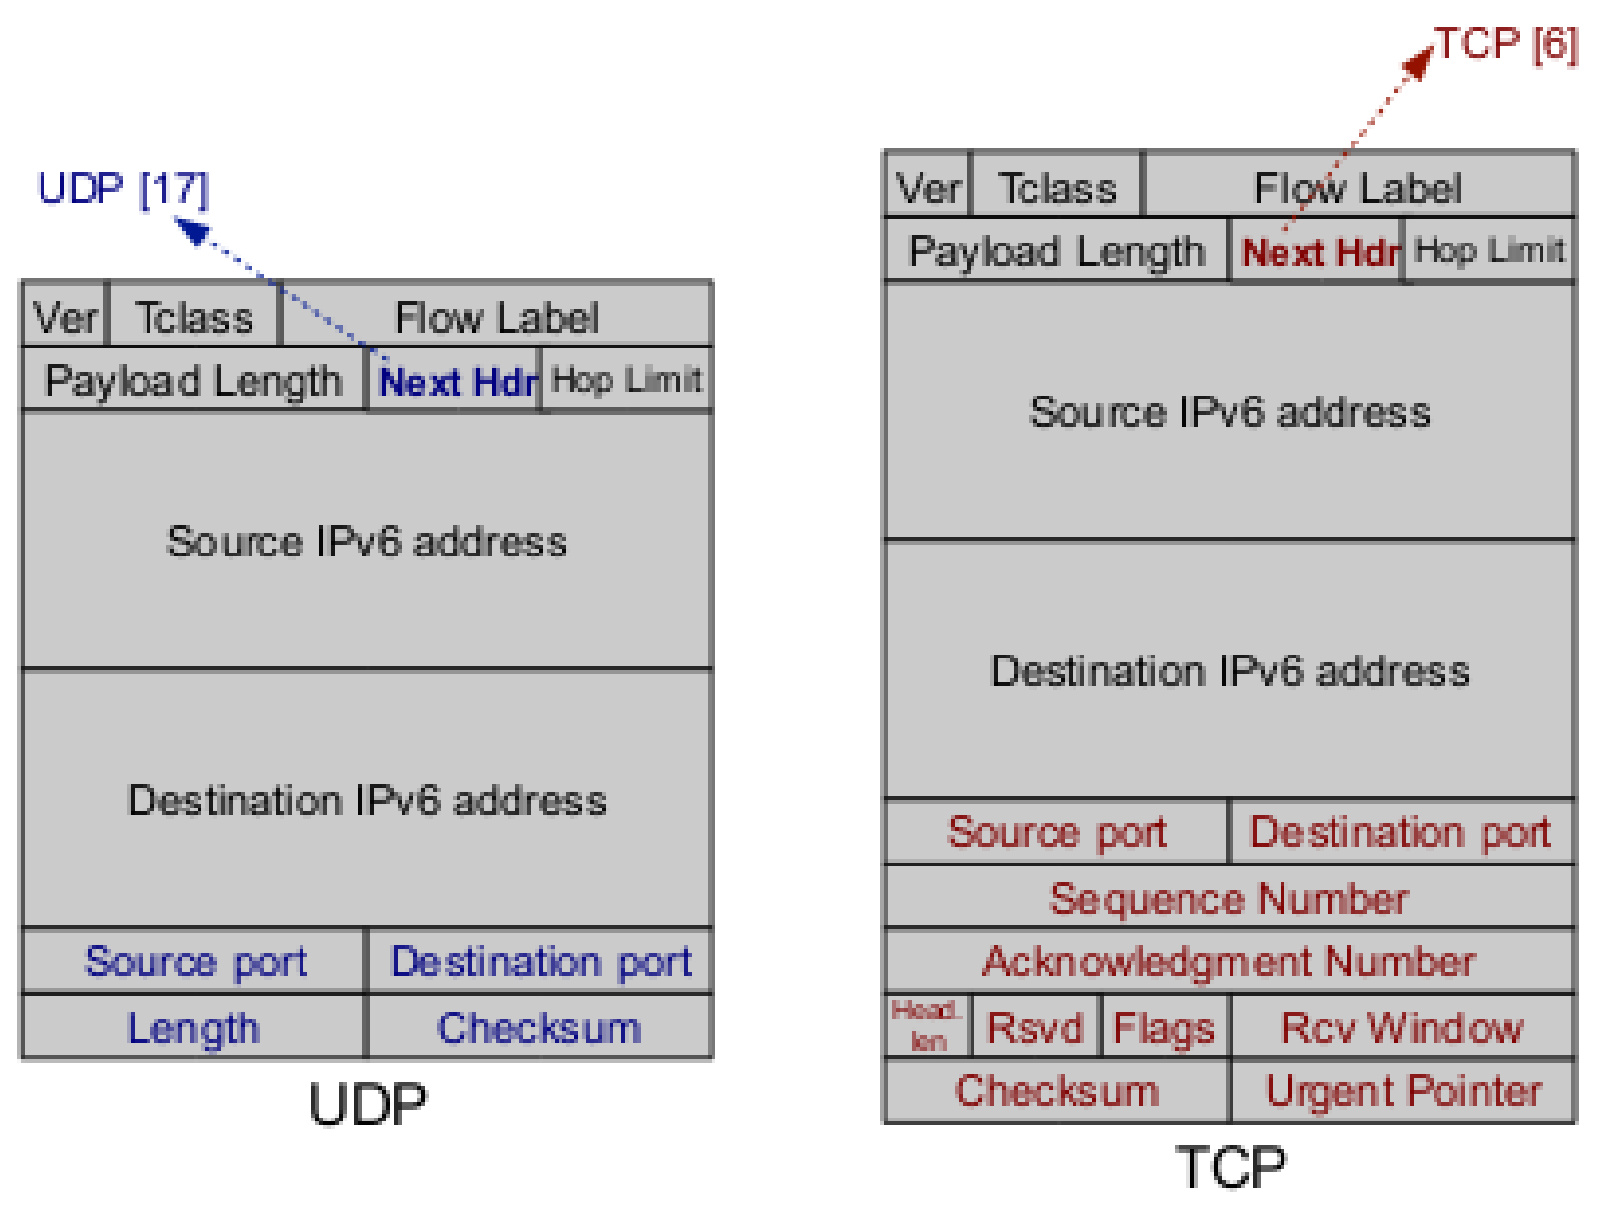
\includegraphics[width=\textwidth]{ipv6format.eps}

\subsection{Extensions du header}

Il est possible de chainer les extensions

\paragraph{Header de routage type 0}

Ce header permet à l'émetteur d'un paquet de spécifier par quels
routeurs doivent passer les paquets. Il permet des attaques et
présente potentiellement des failles de sécurité, bien que la plupart
des appareils supportent cette extension, il est déconseillé de
l'activer en pratique.

\paragraph{Fragmentation des paquets}

Le MTU minimum pour IPv6 est de 1280 bytes et les routeur ne font pas
de fragmentation. Seuls les hosts en bordure fragmentent et
défragmentent les paquets en utilisant un header de
fragmentation. PathMTUDiscovery devrait permettre d'éviter la
fragmentation la plupart du temps.

\section{ICMPv6}

\subsection{Introduction et format des paquets}

\subsection{Auto-configuration}

\subsection{Sécurité}

\section{Support DNS pour IPv6}

\section{Mécanismes de transition}

\chapter{MPLS}

\chapter{Wireless Sensor Networks}

\end{document}
